% Generated from: Zhihu/专栏：概率与统计/渐近统计 (9)：M-估计和 Z-估计_金鱼马_2026-06-15.md
在前面的章节中，我们已经详细介绍了两类经典估计：第~\ref{ch:method-of-moments}~章的矩估计和第~\ref{ch:maximum-likelihood}~章的极大似然估计 (MLE)。

其中，矩估计通过求解矩方程来获得估计值，而 MLE 通过最大化似然函数来寻找最优参数。另一方面，MLE 可以看作求解对数似然方程的解，而广义矩估计将求解参数写作最小化二次型的问题。我们注意到，“通过最大化或最小化函数获得估计值”以及“求解方程获得估计值”似乎可以看作两种基本范式，这正是本章将介绍的 M-估计和 Z-估计；它们提供了一个更加一般化、灵活的参数估计框架。

本章主要参考 van der Vaart~\cite[第 5、19 章]{vandervaart1998}。

\section{M-估计和 Z-估计的基本概念}

M-估计量（M-estimators）由 Peter J. Huber 于 1964 年提出~\cite{huber1964}。

\begin{definition*}[M-估计量与 Z-估计量]
假设 $X_1,X_2,\dots,X_n$ 是取值于概率空间 $(\mathscr X,\mathscr B_x)$ 的随机变量，其总体分布有参数 $\theta$ ------这个 $\theta$ 既可以是参数分布族的参数，也可以在非参数模型下作为总体分布的某个泛函。若一个估计量 $\widehat\theta_n=\widehat\theta_n(X_1,\dots,X_n)$ 最大化某\textbf{\emph{准则函数}} (criterion function) 
$$\theta \mapsto M_n(\theta)=\frac1n\sum_{j=1}^nm_\theta(X_j)$$
那么我们称其为 \textbf{\emph{M-估计量}} ，其中 $m_\theta:\mathscr X\to \overline{\mathbb R}$ 是确定的函数。

s当上式的 $M_n$ （或者说 $m_\theta$ ）可导时，我们自然会通过令导数为零来求解最大化问题。这引出了 \textbf{\emph{Z-估计量}} (Z-estimators) 的概念：其寻找一个估计量 $\widehat{\theta}_n$ 来求解\textbf{\emph{估计方程}} (estimating equations)：
\[\Psi_n(\theta)=\frac1n\sum_{j=1}^n\psi_\theta(X_j)=0\]
其中 $\psi_\theta$ 是确定的向量值函数。一般而言，当 $\theta$ 是 $k$ 维参数时， $\psi_\theta$ 也是一个 $k$ 维函数。
\end{definition*}

\begin{remark}

\begin{itemize}
\tightlist
\item
  M-估计量和 Z-估计量的定义里不要求 $X_1,\dots,X_n$ 是独立同分布 (i.i.d.) 的，即使它们之间存在依赖，仍然可以按照前面的公式，在形式上定义 M 和 Z 估计量。
\item
  如果 $-M_n(\theta)$ 是凸的，那么求解起来更加容易一些，但实际并非总是如此。
\item
  Z-估计可以通过各种数值方法来求解，如（拟）Newton 法、梯度下降、随机梯度下降等等。
\end{itemize}
\end{remark}

在后文中，我们总假设 $X_1,\dots,X_n$ 是 i.i.d. 的，服从分布 $P$ 。对可积函数 $f:\mathscr X\to \mathbb R$ 记
\[
Pf:=\mathbb {E}_P[f(X)]=\int_{\mathscr X}f(x)\mathrm{d}P(x).
\]
再以 $\mathbb P_n$ 代表\emph{经验测度} (empirical measure)，记
\[
\mathbb P_nf:=\frac1n\sum_{j=1}^nf(X_j).
\]
那么
\[
M_n(\theta)=\mathbb P_n m_\theta,\qquad \Psi_n(\theta)=\mathbb P_n\psi_\theta.
\]

我们举几个简单的例子。

\begin{example}[极大似然估计]
设 $X_1, \ldots, X_n$ i.i.d.，有密度函数 $p_\theta(x)$ 。MLE 最大化似然函数 $\prod_{j=1}^n p_\theta(X_j)$，或等价地最大化对数似然函数：
\[
M_n(\theta) := \frac{1}{n}\sum_{j=1}^n \log p_\theta(X_j).
\]

这是一个典型的 M-估计量，其中 $m_\theta(x) = \log p_\theta(x)$。 如果 $X_i$ 不独立，但仍然形式上使用上述式子，求解出的估计量属于所谓的\textbf{\emph{伪似然}} (Pseudo-MLE)。

% \href{https://www.zhihu.com/question/351476933}{如何比较直观地理解 伪极大似然估计（Pesudo-MaximumLikelihood）方法？}


\end{example}

\begin{example}[均值和中位数]
样本均值和样本中位数是两个最基本的位置估计量 (Location estimators)，它们都可以表示为 Z-估计量：

\begin{itemize}
\tightlist
\item
  对样本均值： $\Psi_n(\theta) = \frac{1}{n}\sum_{j=1}^n (X_j - \theta) = 0$ ;
\item
  对样本中位数： $\Psi_n(\theta) = \frac{1}{n}\sum_{j=1}^n \text{sign}(X_j - \theta) = 0$ 。
\end{itemize}


\end{example}

\begin{example}[分位数估计]\label{ex:ch9:quantile}
设 $F$ 是 $\mathbb R$ 上的分布函数，随机变量 $X\sim F$ ，定义其 $\tau$ -分位数 $\theta$ 为所有满足下述关系的实数：\[F(\theta-)=P(X<\theta)\le \tau\le P(X\le \theta)=F(\theta)\]
鉴于在这种定义下分位数可能不唯一（除非 $F$ 处处连续），我们常取如下\textbf{\emph{分位数函数}} 作为 $\tau$ -分位数：
\[
F^{-1}(\tau):=\inf\{x\in\mathbb R:F(x)\ge \tau\},\quad 0<\tau<1.
\]

总体中位数是 $\tau = 0.5$ 的特例。样本分位数大致可以定义为一个点 $\widehat\theta_n$ ，使得 $\tau n$ 部分的样本小于 $\widehat\theta_n$ 而 $(1-\tau)n$ 部分的样本大于 $\widehat\theta_n$ ；一种方法是取 $\widehat\theta_n=\mathbb F_n^{-1}(\tau)$ ，其中 $\mathbb F_n(t):=\frac1n\sum_{j=1}^n\mathbb I(X_j\le t)$ 是经验分布函数。

定义 $$\rho_\tau(y) := y(\tau - \mathbb{I}(y < 0))=y(\tau\mathbb I(y\ge 0)-(1-\tau)\mathbb I(y< 0))$$
这个函数的图像如图~\ref{fig:ch9:quantile-loss-function} 所示。

\begin{figure}[htbp]
  \centering
  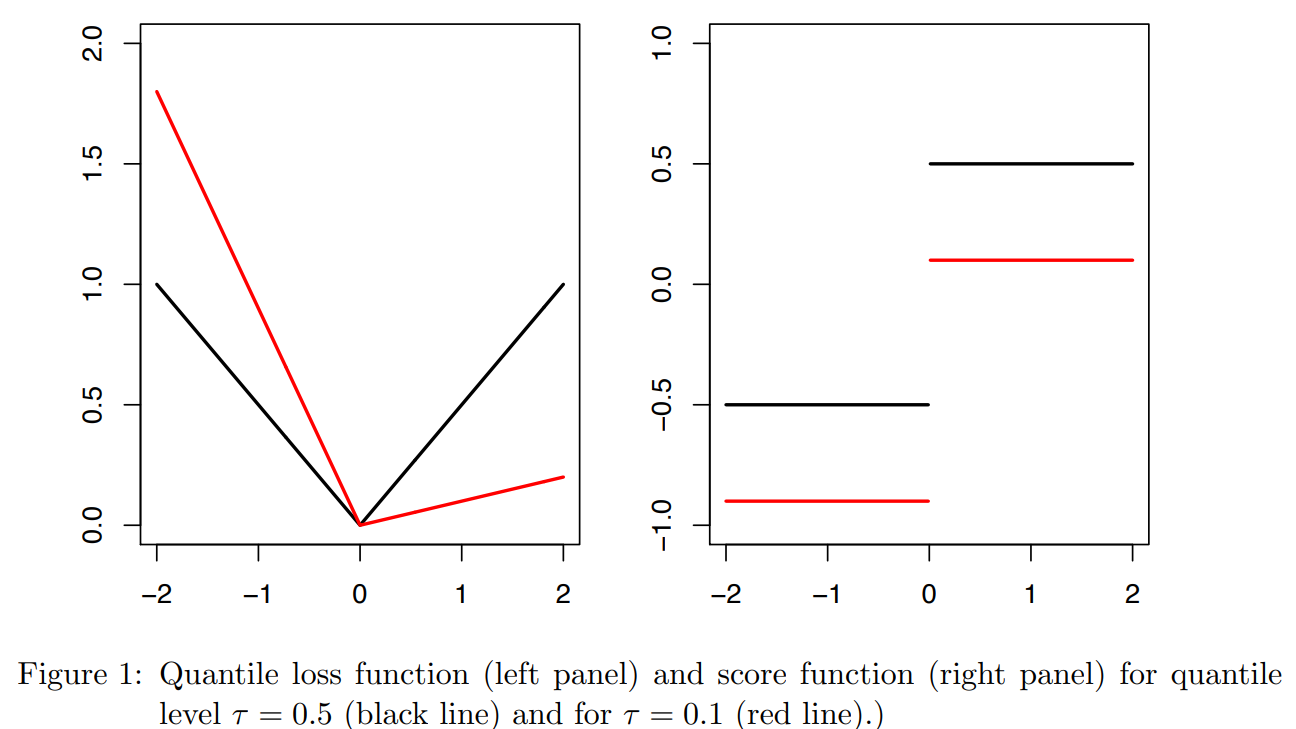
\includegraphics[width=0.58\textwidth]{figures/09-quantile-loss-function.jpg}
  \caption{$\rho_\tau(y)$ 函数的图像，图片来自~\cite{chen2023recursive}。}
  \label{fig:ch9:quantile-loss-function}
\end{figure}

不难证明 $$\operatorname*{\arg\min}_{\theta\in\mathbb R}\mathbb E[\rho_\tau(X-\theta)]=F^{-1}(\tau)$$
从而 $\tau$-样本分位数 $\widehat{\theta}$ 可以表示为 M-估计量：\[M_n(\theta) := \frac{1}{n}\sum_{j=1}^n \rho_\tau(X_j - \theta)\]
对 $\rho_\tau$ 取次导数 (subderivative)，也可以表示为 Z-估计量：\[\Psi_n(\theta) := \frac{1}{n}\sum_{j=1}^n \left((1 - \tau)\mathbb{I}(X_j < \theta) - \tau\mathbb{I}(X_j> \theta)\right) = 0\]
需要说明的是，上述 $\Psi_n(\theta)$ 可能是存在跳跃的，导致 $\Psi_n(\theta)=0$ 无解，如图~\ref{fig:ch9:z-estimator-jump} 所示：

\begin{figure}[htbp]
  \centering
  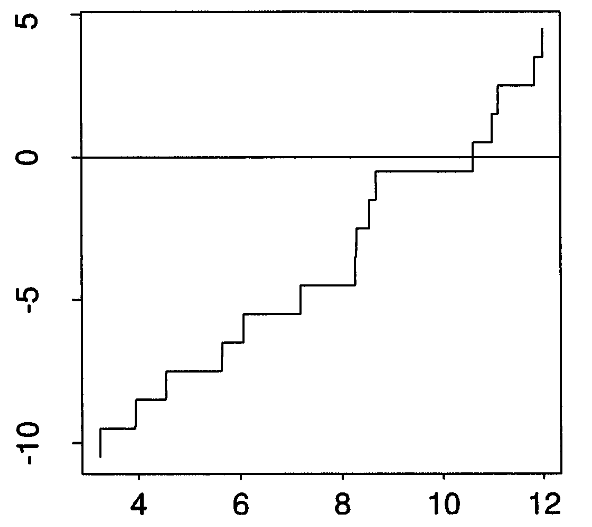
\includegraphics[width=0.58\textwidth]{figures/09-z-estimator-jump.png}
  \caption{从 $\mathrm{Gamma}(5,1)$ 抽取 15 个样本得到的 $\Psi_n(\theta)$。图片来自 \cite{vandervaart1998}, p.~44}
  \label{fig:ch9:z-estimator-jump}
\end{figure}

但也没关系：只要 $n$ 足够大，找一个近似解就已足够。


\end{example}

\begin{example}[Huber 估计量]
Huber 估计量的提出源于鲁棒估计中关于极端数据点对估计影响的研究。众所周知，样本中位数鲁棒但统计效率低、样本均值效率高但对异常值敏感，于是 Huber 估计量试图融合两者的优点。 定义\[\psi(x) = [x]_k := \begin{cases}  -k & \text{若 } x \leq -k \\ x & \text{若 } |x| \leq k \\ k & \text{若 } x \geq k  \end{cases}\]
\textbf{\emph{Huber 估计量}} 求解以下估计方程：
\[
\Psi_n(\theta) = \frac{1}{n}\sum_{j=1}^n \psi(X_j - \theta) = 0.
\]

当数据点距离当前估计值较近（$|X_j- \theta| \leq k$）时，Huber 估计量表现得像均值；当数据点距离较远时，它对异常值的影响进行截断，从而表现得像中位数。参数 $k$ 控制着这个''距离阈值''。

关于 Huber loss 在现代统计学中的应用，感兴趣的读者可以参考 \cite{sunzhoufan2020,hanhuanglinshen2022}。


\end{example}

\section{M 和 Z-估计的相合性}

记参数空间为 $\Theta$ ，配备度量 $d$ ，则相合性指的是 $d(\widehat\theta_n,\theta_0)\overset P\to 0$ ，我们记作 $\widehat\theta_n\overset P\to \theta_0$ 。

\subsection{基本结论}

假设 M-估计 $\widehat\theta_n=\widehat\theta_n(X_1,\dots,X_n)$ 最大化某随机准则函数 $\theta\mapsto M_n(\theta)$ ，即，\[\widehat\theta_n=\operatorname*{\arg\max}M_n(\theta)\]
显然，要想得知 $\widehat\theta_n$ 的渐近行为，必须要考察 $M_n$ 的渐近行为。

首先，我们期望有一个``渐近准则函数'' $\theta\mapsto M(\theta)$ 使得\[M_n(\theta)\overset P\longrightarrow M(\theta),\quad \text{ 当 }n\to\infty,\quad \text{ 对 }\forall \theta\in\Theta\]
当 $M_n(\theta)$ 形如 $\mathbb P_nm_\theta$ 时，可以用大数律直接得出 $M(\theta)=Pm_\theta$ （只要这个期望存在的话）。

真实参数 $\theta_0$ 定义为最大化 $M(\theta)$ 的点：

\[
\theta_0:=\operatorname*{\arg\max}_{\theta\in\Theta}\mathbb E[m_\theta(X)].
\]
非常自然地，我们期望 $M_n$ 的最大值点 $\widehat{\theta}_n$ 能收敛到 $M$ 的最大值点 $\theta_0$。这也是本节首先要证明的东西。不过，要证明这一点，

\begin{itemize}
\tightlist
\item
  $M_n(\theta)\overset P\to M(\theta)$ 的条件有些不太够，至少也要加强到一致收敛，才能保证函数在``形状''上能越来越接近。
\item
  $\theta_0$ 应当是``\textbf{\emph{良分离}} (well separated)''的最大值点。所谓``良分离''是一个比唯一性更强的要求： $M$ 在所有 $d(\theta,\theta_0)\ge\epsilon$ 的点 $\theta$ 处取值都应该能够与 $\theta_0$ 处的值分离开。一个反例如图~\ref{fig:ch9:well-separated} 所示：这个函数有唯一最大值点，但是在无穷远处可能渐近趋近于该最大值，这是我们不愿看到的。
\end{itemize}

\begin{figure}[htbp]
  \centering
  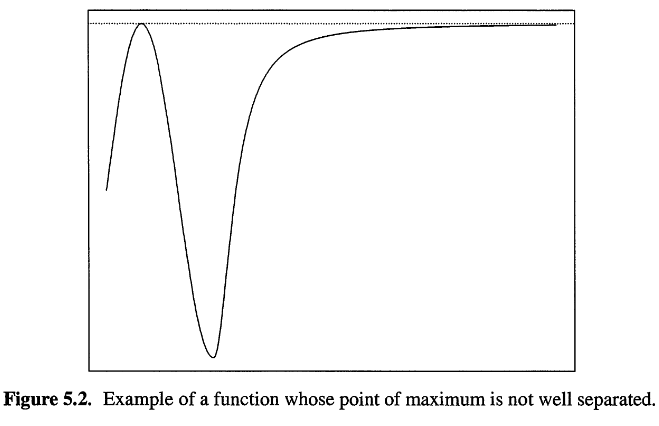
\includegraphics[width=0.68\textwidth]{figures/09-well-separated-maximum.png}
  \caption{唯一但非良分离的最大值点。图片来自 \cite{vandervaart1998}, p.~45}
  \label{fig:ch9:well-separated}
\end{figure}

最后，鉴于找到 $M_n$ 的精确最值可能不容易也不必要，我们只要求找到一个近似的最值作为 $\widehat\theta_n$ ，只需要让 $M_n(\widehat\theta_n)$ 真实最大值的差距是 $o_P(1)$ 的，这称作\textbf{\emph{近似最大条件}} (nearly maximization condition)。

\begin{theorem}[M-估计的相合性]
\label{thm:ch9:m-estimator-consistency}

设 $M_n$ 是随机准则函数而 $M$ 是一个 $\theta$ 的确定函数， $\theta_0=\operatorname*{\arg\max}M(\theta)$ ，假设下面三个条件满足：

\begin{enumerate}
\def\labelenumi{\arabic{enumi}.}
\tightlist
\item
  【一致收敛】 $\sup\limits_{\theta\in\Theta}|M_n(\theta)-M(\theta)|\overset P\to 0$ ；
\item
  【良分离】对每个 $\epsilon>0$ ， $\sup\limits_{\theta\in\Theta,\  d(\theta,\theta_0)\ge\epsilon}M(\theta)<M(\theta_0)$ ；
\item
  【近似最大条件】 $\widehat\theta_n$ 满足 $M_n(\widehat\theta_n)\ge\sup\limits_{\theta\in\Theta}M_n(\theta)-o_P(1)$
\end{enumerate}

那么 $\widehat\theta_n\overset P\longrightarrow \theta_0$ 。

\end{theorem}

\begin{proof}

根据``良分离''条件 (2.)，对任意 $\epsilon>0$，存在 $\eta>0$ 使得
\[
M(\theta)<M(\theta_0)-\eta,\qquad
\forall \theta\in\Theta:\ d(\theta,\theta_0)\ge\epsilon.
\]
若取 $\theta=\widehat\theta_n$，得出 $\big\{d(\widehat\theta,\theta_0)\ge \epsilon\big\}\subset \big\{M(\widehat\theta_n)<M(\theta_0)-\eta\big\}$，即

\begin{equation}
\label{eq:ch9:tag-2}
P\big(d(\widehat\theta_n,\theta_0)\ge\epsilon\big)\le P\big(M(\theta_0)-M(\widehat\theta_n)>\eta\big)
\end{equation}

我们用条件 (3.) 和 (1.) 证明式~\eqref{eq:ch9:tag-2} 右侧收敛于 0：\[ M_n(\widehat\theta_n)\ge\sup\limits_{\theta\in\Theta}M_n(\theta)-o_P(1)\ge M_n(\theta_0)-o_P(1)=M(\theta_0)-o_P(1) \]从而\[M(\theta_0)-M(\widehat\theta_n)\le M_n(\widehat\theta_n)-M(\widehat\theta_n)+o_P(1)\le \sup\limits_{\theta\in\Theta}|M_n(\theta)-M(\theta)|+o_P(1)=o_P(1)\]
于是在式~\eqref{eq:ch9:tag-2} 中取 $n\to\infty$ 即证出 $d(\widehat\theta_n,\theta_0)\overset P\to 0$ 。

\end{proof}

Z-估计的结论和 M-估计如出一辙，只需把定理~\ref{thm:ch9:m-estimator-consistency} 的叙述稍加改动，

\begin{theorem}[Z-估计的相合性]\label{thm:ch9:z-estimator-consistency}

设 $\Psi_n$ 是随机向量值函数， $\Psi$ 是 $\theta$ 的确定向量值函数， $\theta_0$ 满足 $\Psi(\theta_0)=0$ ，假设下面三个条件满足：

\begin{enumerate}
\def\labelenumi{\arabic{enumi}.}
\tightlist
\item
  【一致收敛】 $\sup\limits_{\theta\in\Theta}\|\Psi_n(\theta)-\Psi(\theta)\|\overset P\to 0$ ；
\item
  【良分离】 对每个 $\epsilon>0$ 有 $\inf\limits_{\theta\in\Theta,\ d(\theta,\theta_0)\ge\epsilon}\|\Psi(\theta)\|>0=\|\Psi(\theta_0)\|$ ；
\item
  【近似零条件 (nearly zero condition)】 $\Psi_n(\widehat\theta_n)=o_P(1)$ 。
\end{enumerate}

那么 $\widehat\theta_n\overset P\to \theta_0$ 。

\end{theorem}

\begin{proof}

对 $M_n(\theta)=-\|\Psi_n(\theta)\|$ 和 $M(\theta)=-\|\Psi(\theta)\|$ 用定理~\ref{thm:ch9:m-estimator-consistency}。

\end{proof}

\subsection{更松的相合性条件}

定理~\ref{thm:ch9:m-estimator-consistency} 的良分离可以适当进行修改，得到下述更容易验证的形式：

\begin{theorem}[紧参数空间中的 M-估计相合性]\label{thm:ch9:m-estimator-compact-consistency}

设如下条件成立：

\begin{enumerate}
\def\labelenumi{\arabic{enumi}.}
\tightlist
\item
  【一致收敛】定理~\ref{thm:ch9:m-estimator-consistency} 的条件 (1.)；
\item
  【唯一最大值点】 $M(\theta)=\mathbb E[m_\theta(X)]$ 在 $\theta_0$ 处唯一取得最大值；
\item
  【紧性】参数空间 $\Theta$ 是紧空间；
\item
  【连续性】 $\theta\mapsto M(\theta)$ 连续。
\end{enumerate}

那么，对任意满足

\begin{enumerate}
\def\labelenumi{\arabic{enumi}.}
\setcounter{enumi}{4}
\tightlist
\item
  $M_n(\widehat\theta_n)\ge M_n(\theta_0)-o_P(1)$
\end{enumerate}

的 $\widehat\theta_n$ ，都成立 $\widehat\theta_n\overset P\to \theta_0$ 。

\end{theorem}

\begin{proof}

对任意 $\delta>0$ ，我们记 $B_\delta(\theta_0):=\{\theta:d(\theta,\theta_0)<\delta\}$ 代表 $\theta_0$ 为中心的球。从参数空间中挖去这个球，连续函数 $M$ 在紧集 $\Theta\cap B^c(\theta_0)$ 上有最大值点，记作 $\theta^*$ 。则 (2.) 保证，
$$M(\theta^*)=\sup\limits_{\theta\in\Theta\cap B^c(\theta_0)}M(\theta)<M(\theta_0).$$

下面我们要证明，对任意 $\epsilon>0$ ，当 $n\to\infty$时，下面的式子以趋近于 1 的概率成立

\begin{equation}
\label{eq:ch9:tag-3}
M(\widehat\theta_n)>M_n(\widehat\theta_n)-\frac\epsilon3>M_n(\theta_0)-\frac{2\epsilon}3>M(\theta_0)-\epsilon
\end{equation}

怎么做呢？

\begin{itemize}
\tightlist
\item
  第一个不等号来自于条件 (1.)，一致收敛告诉我们 $P\left(M(\widehat\theta_n)\le M_n(\widehat\theta_n)-\tfrac\epsilon3\right)=o(1)$ ；
\item
  第二个不等号来自于 (5.)，其表明 $P\left(M_n(\widehat\theta_n)\le M_n(\theta_0)-\tfrac\epsilon3\right)=o(1)$ ，或者说， $M_n(\widehat\theta_n)\ge M_n(\theta_0)-o_P(1)>M_n(\theta_0)-\tfrac\epsilon3$ 以趋近于 1 的概率成立；
\item
  第三个不等号与第一个不等号同理。
\end{itemize}

取 $\epsilon=M(\theta_0)-M(\theta^*)>0$ ，代入式~\eqref{eq:ch9:tag-3} 得到：以趋近于 1 的概率\[M(\widehat\theta_n)>M(\theta^*)\]
此时肯定有 $d(\widehat\theta_n,\theta_0)<\delta$ ，因 $M(\theta^*)$ 是 $\Theta\cap B^c(\theta_0)$ 中的最大值；由 \[ 1\leftarrow P\big(M(\widehat\theta_n)>M(\theta^*)\big)\le P\big(d(\widehat\theta_n,\theta_0)<\delta\big)\le 1 \]知 $n\to\infty$ 时， $P\big(d(\widehat\theta_n,\theta_0)<\delta\big)\to 1$ ，从而证明了结论。

\end{proof}

接下来我们把目光放在``一致收敛''这个条件上。一致收敛可以由如下概念进行刻画：

\begin{definition*}[Glivenko--Cantelli 类]
一族可测函数 $\mathscr F$ 若满足 $\|\mathbb P_n-P\|_{\mathscr F}:=\sup\limits_{f\in\mathscr F}|\mathbb P_nf-Pf|\to 0\quad \text{a.s.}$，
则称 $\mathscr F$ （关于 $P$ ）是一个 \textbf{\emph{Glivenko-Cantelli 类}} (Glivenko-Cantelli class)，简称 GC 类。
\end{definition*}

当 $M_n(\theta)=\mathbb P_n m_\theta$ 、 $M(\theta)=Pm_\theta$ 时，`` $M_n(\theta)$ 一致收敛到 $M(\theta)$ ''实际上是在要求 $\{m_\theta:\theta\in\Theta\}$ 构成一个 GC 类；一个充分条件如下：

\begin{proposition}[一致大数律的一个充分条件]
\label{prop:ch9:gc-sufficient-condition}
设 $\Theta$ 是紧度量空间，对每个 $x\in\mathscr X$，函数 $\theta\mapsto m_\theta(x)$ 都是 a.s. 连续的，且这些 $m_\theta(x)$ 都被某可积函数控制，那么 $\{m_\theta:\theta\in\Theta\}$ 是 GC 类。
\end{proposition}

上述结论称作\emph{一致大数律} (ULLN)。

% \href{https://www.zhihu.com/question/387169516/answer/1147878576}{谁可以解释一下``一致大数定律''?}

Z-估计的情况是相同的，设 $\psi_\theta=(\psi_{\theta,1},\dots,\psi_{\theta,k})^\top$ ，那么 $\Psi_n(\theta)=\mathbb P_n\psi_\theta$ 一致收敛到 $\Psi(\theta)=P\psi_\theta$ ，实际上是在要求 $\{\psi_{\theta,i},\theta\in\Theta,i=1,\dots,k\}$ 构成 GC 类。

但是，一致收敛这个条件其实过于强了，并且在实际中很难去验证。如果想更精细地刻画一致收敛，往往需要借助经验过程 (Empirical Process) 的工具，建议读者参考 \cite{vandervaartwellner1996}、\cite{geer2000}。

下面的定理提供了 Z-估计相合、不要求一致收敛的情形，来自 \cite{vandervaart1998} 一书 Lemma 5.10 (p.47)，

\begin{theorem}[单调 Z-估计的相合性]\label{thm:ch9:monotone-z-consistency}

设 $\Theta\subset\mathbb R$ ， $\Psi_n$ 是随机函数， $\Psi$ 是 $\theta$ 的确定函数， $\Psi_n(\theta)\overset P\to\Psi(\theta)$ 对每个 $\theta\in\Theta$ 成立（逐点收敛），设有如下条件，

\begin{enumerate}
\def\labelenumi{\arabic{enumi}.}
\tightlist
\item
  如下条件其中之一成立：
\end{enumerate}

\begin{itemize}
\tightlist
\item
  对每个 $\theta\in\Theta$ ，函数 $\theta\mapsto \Psi_n(\theta)$ 连续，并且有唯一的零点 $\widehat\theta_n$ ；
\item
  对每个 $\theta\in\Theta$ ，函数 $\theta\mapsto \Psi_n(\theta)$单调非降，且 $\Psi_n(\widehat\theta_n)=o_P(1)$ ；
\end{itemize}

\begin{enumerate}
\def\labelenumi{\arabic{enumi}.}
\setcounter{enumi}{1}
\tightlist
\item
  $\theta_0$ 满足：对任意 $\epsilon>0$ ， $\Psi(\theta_0-\epsilon)<0<\Psi(\theta_0+\epsilon)$ 。
\end{enumerate}

那么 $\widehat\theta_n\overset P\to \theta_0$ 。

\end{theorem}

\begin{proof}

如果 $\theta\mapsto \Psi_n(\theta)$ 连续且有唯一的零点 $\widehat\theta_n$ ，那么事件 $\{\Psi_n(\theta_0-\epsilon)<0<\Psi_n(\theta_0+\epsilon)\}$ 蕴含 $\theta_0-\epsilon<\widehat\theta_n<\theta_0+\epsilon$ ，即， 
$$P\Big(\Psi_n(\theta_0-\epsilon)<0<\Psi_n(\theta_0+\epsilon)\Big)\le P\big(\theta_0-\epsilon<\widehat\theta_n<\theta_0+\epsilon\big)$$
上式左侧是收敛于 1 的，因为 $\Psi_n(\theta_0\pm\epsilon)\overset P\to\Psi(\theta_0\pm\epsilon)$ ，从而上式右侧也收敛于 1，这证明了 $\widehat\theta_n\overset P\to\theta_0$ 。

下面证明 $\theta\mapsto \Psi_n(\theta)$ 单调非降的情形。对每个 $\eta>0$ ，当 $\Psi_n(\theta_0-\epsilon)<-\eta$ 成立时，由单调性，若 $\widehat\theta_n\le\theta_0-\epsilon$ ，则 
$\Psi_n(\widehat\theta_n)\le\Psi_n(\theta_0-\epsilon)<-\eta$ ，即 
$$\{\Psi_n(\theta_0-\epsilon)<-\eta\}\cap \{\widehat\theta_n\le\theta_0-\epsilon\}\subset \{\Psi_n(\widehat\theta_n)<-\eta\}$$

从而 $$P(\Psi_n(\theta_0-\epsilon)<-\eta)\le P(\widehat\theta_n>\theta_0-\epsilon)+\underbrace{P(\Psi_n(\widehat\theta_n)<-\eta)}_{o(1)}$$

另一个方向同理，于是对每个 $\epsilon,\eta>0$ ，\[\begin{aligned} P\big(\Psi_n(\theta_0-\epsilon)<-\eta,\Psi_n(\theta_0+\epsilon)>\eta\big) \le P\big(\theta_0-\epsilon<\widehat\theta_n<\theta_0+\epsilon\big)+o(1) \end{aligned}\]
取 $2\eta=\min\{-\Psi(\theta_0-\epsilon),\Psi(\theta_0+\epsilon)\}$ 则上式左侧收敛于 1。

\end{proof}

\begin{example}[样本中位数的相合性]\label{ex:ch9:median-consistency}
设 $\mathbb R$ 上的随机变量 $X\sim F$ ，其中 $F$ 有唯一的总体中位数 $\theta_0$ ，这里的``唯一''是指对任意 $\epsilon>0$ ，
\[
P(X<\theta_0-\epsilon)<0.5<P(X<\theta_0+\epsilon).
\]
样本中位数 $\widehat\theta_n$ 作为 Z-估计可以写作下述方程的解：
\[
\Psi_n(\theta)=\frac1n\sum_{j=1}^n\mathrm{sign}(X_j-\theta).
\]

根据大数律，对每个 $\theta$ ， 
$$\Psi_n(\theta)\overset P\to \Psi(\theta)=\mathbb{E}[\mathrm{sign}(X-\theta)]=P(X>\theta)-P(X<\theta)$$
容易验证：

\begin{itemize}
\tightlist
\item
  $\theta\mapsto-\Psi_n(\theta)$ 单调非降；
\item
  $-\Psi(\theta_0-\epsilon)<0<-\Psi(\theta_0+\epsilon)$ 。
\end{itemize}
那么根据定理~\ref{thm:ch9:monotone-z-consistency}， $\widehat\theta_n\overset P\to \theta_0$ 。

\end{example}

类似于前面的中位数例子，请读者结合分位数估计的例子和定理~\ref{thm:ch9:monotone-z-consistency} 自行证明：如果 $F$ 有唯一的 $\tau$ 分位数 $F^{-1}(\tau)$ ，则样本 $\tau$ -分位数 $\mathbb F_n^{-1}(\tau)$ 也是相合估计。


\subsection{Wald 的相合性证明}

本节中我们介绍另一组条件，来自 Wald 在 1949 年对 MLE 的相合性证明，这里既不需要一致收敛，也放宽了连续性、紧性，从而提供了一个更一般的框架。

首先引入一个比连续性更弱的概念：\emph{\textbf{\href{https://en.wikipedia.org/wiki/Semi-continuity}{半连续性}} }。

\begin{definition*}[半连续性]
实值函数 $f$ 如果满足\[\limsup_{x \to x_0} f(x) \leq f(x_0)\]
则称其在点 $x_0$ 处\textbf{\emph{上半连续}} （upper semi-continuous, u.s.c.）；如果\[\liminf_{x \to x_0} f(x) \geq f(x_0)\]
则称其在点 $x_0$ 处\textbf{\emph{下半连续}} （lower semi-continuous, l.s.c.）。
\end{definition*}

图~\ref{fig:ch9:semicontinuity} 直观展示了上半连续与下半连续的区别\footnote{注意，上/下半连续与左/右连续没有任何关系。}。

\begin{figure}[htbp]
  \centering
  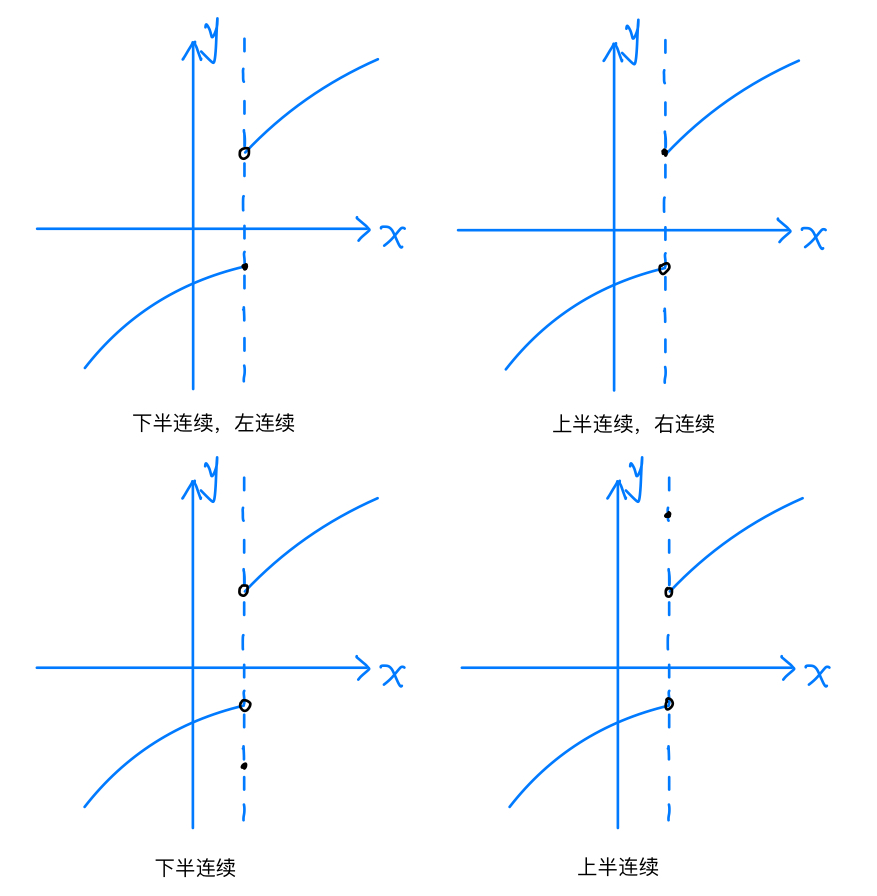
\includegraphics[width=0.62\textwidth]{figures/09-semicontinuity.png}
  \caption{上半连续与下半连续的示意图。图片来自 \url{https://www.cnblogs.com/BoyaYan/p/17237330.html}}
  \label{fig:ch9:semicontinuity}
\end{figure}

% （注意，上/下半连续与左/右连续没有任何关系。）%，例子见 \url{https://math.stackexchange.com/q/3884576}。）

对函数 $\theta\mapsto Pm_\theta=\mathbb{E}_P[m_\theta(X)]$ ，之前的假设都是它有唯一的最大值点 $\theta_0$ 。但在这里，我们允许它有多个最大值点，并记 \[ \Theta_0:=\big\{\theta_0\in\Theta:Pm_{\theta_0}=\sup\nolimits_\theta Pm_\theta\big\}\ne\varnothing \]代表所有能取到最大值的点集。

\begin{theorem}[Wald 相合性]\label{thm:ch9:wald-consistency}

设如下三个条件满足，

\begin{enumerate}
\def\labelenumi{\arabic{enumi}.}
\tightlist
\item
  【u.s.c.】 对每个 $\theta\in\Theta$ ， $\theta\mapsto m_\theta(x)$ a.s. 是上半连续的，即 $\limsup\limits_{\theta_n\to\theta}m_{\theta_n}(x)\le m_\theta(x),\quad \text{a.s.}$ (这里``a.s.''的例外集允许依赖于 $\theta$ 。)
\item
  【局部一致可积】 对每个球 $U\subset\Theta$ ，函数 $x\mapsto \sup\limits_{\theta\in U}m_\theta(x)$ 可测，且满足
  \[
  P\sup_{\theta\in U}m_\theta(x)=\mathbb E_P\left[\sup_{\theta\in U}m_\theta(X)\right]<\infty.
  \]
\item
  【近似最大条件】存在某个 $\theta_0\in\Theta_0$ 使得 $M_n(\widehat\theta_n)\ge M_n(\theta_0)-o_P(1)$ 。
\end{enumerate}

那么，对任意 $\epsilon>0$ 和紧集 $K\subset\Theta$ ，
\[
P(d(\widehat\theta_n,\Theta_0)\ge\epsilon,\ \widehat\theta_n\in K)\to 0.
\]

即， $\widehat\theta_n$ 落在紧集 $K$ 内但与 $\Theta_0$ 内每个点的距离都不低于 $\epsilon$ 的概率趋于 0。

\end{theorem}

\begin{proof}

记集合 $B := \{\theta \in K : d(\theta, \Theta_0) \geq \varepsilon\}$，我们要证明 $P(\widehat{\theta}_n \in B) \to 0$。

首先，如果函数 $\theta \mapsto Pm_\theta$ 恒等于 $-\infty$ ，则 $\Theta_0 = \Theta$，结论平凡成立。否则，我们可以假设存在 $\theta_0\in\Theta_0$ 使得 $Pm_{\theta_0} > -\infty$ ；那么由条件 (2.)， $\mathbb{E}_P[|m_{\theta_0}(X)|]<\infty$ 。

固定某个 $\theta \in K$，令 $U_l \downarrow \theta$ 为围绕 $\theta$ 的直径趋于零的递减开球列。记 $m_U(x) := \sup_{\theta\in U} m_\theta(x)$ ，则对每个 $l$， $m_{U_l}(x)$ 关于 $l$ 递减，且 $m_\theta(x) \leq m_{U_l}(x),\quad \forall\, l$

取 $l\to\infty$ ，

\begin{itemize}
\tightlist
\item
  一方面 $m_\theta(x)\le \lim\limits_{l\to\infty}m_{U_l}(x)$ ；
\item
  令一方面 $U_l$ 收缩到 $\theta$ ，再结合 $m_\theta(x)$ 的上半连续性 (1.)， $\lim\limits_{l\to\infty} m_{U_l}(x) \leq m_\theta(x)$ a.s.。
\end{itemize}

从而 $\lim\limits_{l\to\infty} m_{U_l}(x) = m_\theta(x)$ ，即 $m_{U_l} \downarrow m_\theta$ a.s.。
对函数列 $\{-m_{U_l}\}$ 用单调收敛定理，有 \footnote{这里的右侧可能是 $-\infty$ 。}

$$\mathbb{E}[m_{U_l}(X)] \to \mathbb{E}[m_\theta(X)] ,\quad \text{ 当 }l\to\infty$$


当 $\theta\not\in\Theta_0$ 时，由于 $\mathbb{E}[m_{U_l}(X)] \to \mathbb E[m_\theta(X)]<\mathbb E[m_{\theta_0}(X)]$ ，故在序列 $\{U_l\}$ 中总存在一个包含 $\theta$ 的开球 $U_\theta$ 使得

\begin{equation}
\label{eq:ch9:tag-4}
\mathbb E[m_{U_\theta}(X)]<\mathbb E[m_{\theta_0}(X)]
\end{equation}

注意到$\{U_\theta : \theta \in B\}$ 构成 $B$ 的一个开覆盖，由于 $K$ 是紧集，其闭子集 $B \subset K$ 也是紧集，故存在有限子覆盖 $U_{\theta_1}, \dots, U_{\theta_p}$。由大数律 ，

\begin{equation}
\label{eq:ch9:tag-5}
\begin{aligned} \sup_{\theta\in B}\mathbb P_nm_\theta&\le\max_{i=1,\dots,p}\sup_{\theta\in U_{\theta_i}} \mathbb P_nm_\theta\\ &\le \max_{i=1,\dots,p}\mathbb P_n\sup_{\theta\in U_{\theta_i}}m_\theta\\ &\xrightarrow{\text{a.s.}}\max_{i=1,\dots,p}\mathbb{E}\left[\sup_{\theta\in U_{\theta_i}}m_\theta(X)\right]\\ &<\mathbb{E}[m_{\theta_0}(X)] \end{aligned}
\end{equation}

其中最后一行来自式~\eqref{eq:ch9:tag-4} 。

另一方面，如果 $\widehat\theta_n\in B$ ，那么根据条件 (3.) 和大数律\[ \sup_{\theta \in B} \mathbb{P}_n m_\theta \geq \mathbb{P}_n m_{\widehat{\theta}_n} \geq \mathbb{P}_n m_{\theta_0} - o_P(1) = \mathbb{E}[m_{\theta_0}(X)]-o_P(1) \]

这表明事件 $\{\widehat{\theta}_n \in B\}$ 蕴含 $\sup\limits_{\theta\in B} \mathbb{P}_n m_\theta \ge \mathbb{E}[m_{\theta_0}(X)] - o_P(1)$。结合式~\eqref{eq:ch9:tag-5} ，\[P(\widehat\theta_n\in B)\le P\left(\sup_{\theta\in B}\mathbb P_nm_\theta\ge\mathbb E[m_{\theta_0}(X)]-o_P(1)\right)\to 0\]
\end{proof}

\begin{remark}

\begin{itemize}
\tightlist
\item
  为了应用此定理，参数空间 $\Theta$ 最好是紧的；不然的话，应当额外表明 $\widehat\theta_n$ 最终会落入某个紧集，或者对参数空间进行合适的紧化 (compactification)。
\item
  一种方法是对 $m_\theta$ 施加强制条件 (Coercivity condition)，即当 $|\theta|\to\infty$ 时 $m_\theta\to -\infty$ ，从而 $\widehat\theta_n$ 总是胎紧的，其概率集中在某个紧集内。
\item
  虽然 $\mathbb R$ 在通常拓扑下不是紧空间，但是我们可以加入两个点 $\overline{\mathbb R}:=\mathbb R\cup\{-\infty,\infty\}$ 构成扩展实数轴。 $\arctan$ 是 $\overline{\mathbb R}$ 到闭区间 $\left[-\tfrac\pi2,\tfrac\pi2\right]$ 的一个同胚，从而 $\overline{\mathbb R}$ 就是一个紧度量空间，其度量可取 $d(x,y)=|\arctan x-\arctan y|$ 。
\end{itemize}
\end{remark}

\begin{example}[Cauchy 似然]
Cauchy 分布 $\text{Cauchy}(\theta)$ 的 PDF 为
\[
p_\theta(x)=\frac1{\pi(1+(x-\theta)^2)},\quad x\in\mathbb R.
\]
其中 $\theta$ 是位置参数，我们取参数空间为扩展实数轴 $\Theta=\overline{\mathbb R}$ 。

设有 i.i.d. 样本 $X_1,\dots,X_n$ ，则 $\theta$ 的 MLE 最大化 $\theta\mapsto\mathbb P_nm_\theta$ ，其中， 
$$m_\theta(x)=-\log(1+(x-\theta)^2)$$
特别地，定义\[\begin{aligned} m_{-\infty}(x)&=\limsup_{\theta\to-\infty}m_\theta(x)=-\infty\\ m_{\infty}(x)&=\limsup_{\theta\to\infty}m_\theta(x)=-\infty\\  \end{aligned}\]
我们验证一下定理~\ref{thm:ch9:wald-consistency} 的条件：

\begin{enumerate}
\def\labelenumi{\arabic{enumi}.}
\tightlist
\item
  首先 $m_\theta(x)$ 是连续的，自然上半连续；
\item
  局部一致可积：对 $U\subset \Theta$ ，
  \[
  \mathbb E\left[\sup_{\theta\in U}m_\theta(X)\right]=\int_{\mathbb R}\sup_{\theta\in U}\frac{-\log(1+(x-\theta)^2)}{\pi(1+(x-\theta)^2)}{\rm d}x<\infty.
  \]
\item
  $\widehat\theta_n$ 是 MLE，自然满足 $M_n(\widehat\theta_n)=\sup\limits_{\theta\in\Theta}M_n(\theta)\ge M_n(\theta_0)-o_P(1)$ 。
\end{enumerate}
由可识别性， $\Theta_0=\{\theta_0\}$ ，故定理~\ref{thm:ch9:wald-consistency} 给出 $\widehat\theta_n\overset P\to \theta_0$ 。


\end{example}

\section{M 和 Z-估计的渐近正态性}

\subsection{经验过程与 Donsker 类}

要证明渐近正态性，我们不得不引入一些经验过程的工具。如果读者不想看这些东西，大可以跳过本节，只需承认本节末尾的式~\eqref{eq:ch9:tag-6} 成立就可以。

设 $X_1,\dots,X_n$ 是来自分布 $P$ 的 i.i.d. 样本， $\mathbb P_n=\frac1n\sum_{j=1}^n\delta_{X_j}$ 是经验测度。定义\href{https://en.wikipedia.org/wiki/Empirical_process}{经验过程} (Empirical process)\[\mathbb G_n:=\sqrt n(\mathbb P_n-P)\]
我们可以将 $\mathbb G_n$ 看作是一个符号测度，用于衡量经验分布与真实分布的差距。对可积函数 $f:\mathscr X\to\mathbb R$ ，定义经验过程在 $f$ 处的取值为 
$$\mathbb G_nf=\sqrt n(\mathbb P_nf-Pf)=\sqrt n\left(\frac1n\sum_{j=1}^n\ f(X_j)-\mathbb E[f(X)]\right)$$s
给定一族 $\mathscr X\to \mathbb R$ 的 $P$ -可积函数 $\mathscr F$ ，则上述 $P$ 、 $\mathbb P_n$ 和 $\mathbb G_n$ 又都可以视作 $\mathscr F\to \mathbb R$ 的算子。

记 $\ell^\infty(\mathscr F)$ 是所有 $\mathscr F\to \mathbb R$ 的有界算子构成的 Banach 空间：
\[
x\in \ell^\infty(\mathscr F)\quad \iff \quad \sup_{f\in\mathscr F}|x(f)|<\infty.
\]
如果函数族 $\mathscr F$ 满足
\[
\sup_{f\in\mathscr F}|f(x)-Pf|<\infty,\qquad \forall x\in\mathscr X,
\]
那么 $\mathbb G_n$ 还可以视作从 $\ell^\infty (\mathscr F)$ 中取值的随机元。
$$\mathbb G_n:\omega\mapsto \sqrt n\left(\frac1n\sum_{j=1}^nf(X_j(\omega))-\mathbb{E}[f(X)]\right)$$
我们考察其在 $\ell^\infty(\mathscr F)$ 中的极限：
\begin{definition*}[Donsker 类]
若存在 $\ell^\infty(\mathscr F)$ 中 Borel-可测的、胎紧的随机元 $\mathbb G_P$，使得 $\mathbb G_n$ 在 $\ell^\infty(\mathscr F)$ 中弱收敛到 $\mathbb G_P$，那么称 $\mathscr F$ 是一个 \textbf{\emph{Donsker 类}}，或者 $P$-Donsker 类。
\end{definition*}

当每个 $f$ 平方可积（即 $Pf^2<\infty$ ）时，由经典中心极限定理， $\mathbb G_n f\overset{\rm d}\to \mathcal N(0,\mathrm{Var}[f(X)])$ ；Donsker 类就建立在这种观察上，它的定义本质上是在说``使得这种弱收敛成立的那些函数族''。

我们对比一下 GC-类和 Donsker 类，

\begin{itemize}
\tightlist
\item
  Glivenko-Cantelli (GC) 类对应的是一致的大数律，它保证了经验均值 $\mathbb{P}_n f$ 在整个函数族上都一阶收敛到真实期望 $Pf$。
\item
  Donsker 类对应的是一致的中心极限定理，它保证经验过程 $\mathbb G_n$ 在 $\ell^\infty(\mathscr F)$ 中整体弱收敛到一个极限随机元 $\mathbb G_P$ 。
\end{itemize}

这个极限元 $\mathbb G_P$ 是一个零均值 \textbf{\emph{Gaussian 过程}} ，这指的是，对每个 $k=1,2,\dots<\infty$ 和任意 $f_1,\dots ,f_k\in\mathscr F$ ， 
$$(\mathbb G_P f_1,\mathbb G_P f_2,\dots,\mathbb G_Pf_k)\sim \mathcal N_k(\mathbf{0},\Sigma)$$
其中 $\Sigma$ 是 $k\times k$ 矩阵，其 $i,j$ 元为 $P(f_i-P f_i)(f_j-Pf_j)=\mathrm{Cov}_{X\sim P}[f_i(X),f_j(X)]$ 。

\begin{example}[Brownian 桥]
记分布函数 $F(t)=P(X\le t)$ 和经验分布函数 $\mathbb F_n(t)=\mathbb P_n(X\le t)$，$\mathscr F=\{\mathbb I(\cdot \le t)\}_{t\in\mathbb R}$。
\end{example}

\begin{theorem}[Donsker--Skorokhod--Kolmogorov 定理]
\label{thm:ch9:donsker}
函数类 $\mathscr F$ 是 Donsker 类，且 $\mathbb G_n(t)=\sqrt n(\mathbb F_n(t)-F(t))\overset{\rm d}\to \mathbb G_P(t)$。
\end{theorem}

其中 $\mathbb G_P(t)$称作 $P$ -\textbf{\emph{Brownian 桥}} ，这是一个 Gaussian 过程，且由于对 $s,t\in\mathbb R$ 有 $\mathbb E[\mathbb I(X\le s)\mathbb I(X\le t)]=F(s\wedge t)$ ，故
\[
\mathrm{Cov}[\mathbb G_P(t),\mathbb G_P(s)]=F(s\wedge t)-F(s)F(t).
\]

\begin{remark}

\begin{itemize}
\tightlist
\item
  上例中的弱收敛可以视作是在 $\ell^\infty(\overline{\mathbb R})$ 中的收敛，也可以视作是在其子空间： \href{https://en.wikipedia.org/wiki/Skorokhod_space}{Skorokhod 空间} $\mathcal D(-\infty,\infty)$ 中的收敛。当配备上确界范数 $\|\cdot\|_\infty$ 时，选择哪个空间并不影响结论。
\item
  最早是由 Donsker 于 1952 年对 $[0,1]$ 上的均匀分布证明了这一结论，一个证明可以参考 \cite{linluzhang2023} 一书的 §8.3。
\end{itemize}
\end{remark}

\begin{example}[Lipschitz 函数类]\label{ex:ch9:lipschitz-function}
设 $\Theta\subset\mathbb R^d$ 紧， $\mathscr F=\{f(x,\theta)\}_{\theta\in\Theta}$ ，其中 $f:\mathscr X\times \Theta\to\mathbb R$ 。设对每个 $x$ ， $f(x,\cdot)$ 是 $L(x)$ -Lipschitz 的，即 $|f(x,\theta_1)-f(x,\theta_2)|\le L(x)\|\theta_1-\theta_2\|$

如果 $L(x)$ 是平方可积的，那么可以证明 $\mathscr F$ 是 Donsker 类： 
$$\mathbb G_n(\theta)=\sqrt n(\mathbb P_nf(\theta,\cdot)-Pf(\theta,\cdot))\overset{\rm d}\to \mathbb G(\theta)$$
其中 
$$\mathrm{Cov}(\mathbb G(\theta_0),\mathbb G(\theta_1))=\mathrm{Cov}_{X\sim P}[f(X,\theta_0),f(X,\theta_1)]$$


\end{example}
这两个例子也可参考 \cite{duchi2018stats300b15}。

下面证明一个非常有用的引理，来自 \cite{vandervaart1998} 的 Lemma 19.24。它说的是：如果我们用 $\mathscr F$ 中的一列函数 $\widehat f\!_n$ 去逼近某个 $f_0$ ，那么经验过程作用在 $\widehat f\!_n$ 上和作用在 $f_0$ 上的效果相同。这相当于``用相合估计量替换参数不会改变渐近分布''。


\begin{lemma}[Donsker 类中的随机替换]\label{lem:ch9:donsker-random-substitution}

设 $\mathscr{F}$ 是一族可测函数的 $P$ -Donsker 类， $\{\widehat{f}\!_n\}$ 为一列在 $\mathscr{F}$ 中取值的随机元，使得对某个 $f_0\in L^2(P)$ （即 $Pf_0^2<\infty$ ）有
\[
\int_{\mathscr X} (\widehat{f}_n(x) - f_0(x))^2 \,\mathrm{d}P(x) = P(\widehat{f}\!_n - f_0)^2 \overset{P}{\to} 0.
\]

则 $\mathbb G_n(\widehat f\!_n-f)\overset P\to 0$ ，从而， $\mathbb G_n\widehat f\!_n\overset{\rm d}\to \mathbb G_P f_0$ 。

\end{lemma}

\begin{proof}

不失一般性，可以假设 $f_0\in\mathscr F$ ，否则用 $\mathscr F\cup\{f_0\}$ 替换 $\mathscr F$ 仍然保持 Donsker 类。考虑
\[
g:\ell^\infty(\mathscr F)\times\mathscr F\to\mathbb R,\quad g(z,f)=z(f)-z(f_0).
\]

为 $\mathscr F$ 赋予 $L_2(P)$ 度量，那么只要 $f\mapsto z(f)$ 在 $f$ 处连续， $g$ 在 $(z,f)$ 就在乘积空间中是连续的。这是因为：若在 $\ell^\infty(\mathscr F)\times\mathscr F$ 中 $(z_n,f_n)\to (z,f)$ ，则 $z_n$ 一致收敛到 $z$ ，故若 $z$ 在 $f$ 处连续时
\[
z(f_n)=z(f)+o(1)\longrightarrow z(f).
\]
由引理中的条件， $\widehat f\!_n$ 在 $L_2(P)$ 下收敛到 $f_0$ ，这蕴含了在 $(\mathscr F,L_2(P))$ 中的依概率收敛 $\widehat f\!_n\overset P\to f_0$ 。又由于 $\mathscr F$ 是 $P$ -Donsker 类，在 $\ell^\infty(\mathscr F)$ 中有 $\mathbb G_n\overset{\rm d}\to \mathbb G_P$ 。二者结合，在 $\ell^\infty(\mathscr F)\times \mathscr F$ 中，
\[
(\mathbb G_n,\widehat f\!_n)\overset{\rm d}\to (\mathbb G_P,f_0).
\]

Gaussian 过程 $\mathbb G_P$ 的轨道在 $\mathscr F$ 上几乎处处连续， 从而， $g$ 在几乎每个点 $(\mathbb G_P,f_0)$ 处连续。由连续映射定理，
\[
\mathbb G_n\big(\widehat f\!_n-f_0\big)=g(\mathbb G_n,\widehat f\!_n)\overset{\rm d}\to g(\mathbb G_P,f_0)=0.
\]

\end{proof}

设 $\widehat{f}\!_n := \psi_{\widehat{\theta}_n}$，$f_0 := \psi_{\theta_0}$，且存在平方可积的 $\dot{\psi}$ 使得，\[P(\psi_{\widehat{\theta}_n} - \psi_{\theta_0})^2 \leq P(\dot{\psi}^2) \|\widehat{\theta}_n - \theta_0\|^2 = O_P(\|\widehat{\theta}_n - \theta_0\|^2)\]
如果 $\widehat{\theta}_n \overset{P}{\to} \theta_0$，则上式趋于 0。因此，只要函数类 $\{\psi_\theta\}$ 是 $P$ -Donsker 的，根据引理~\ref{lem:ch9:donsker-random-substitution}，我们就有\[\mathbb{G}_n(\psi_{\widehat{\theta}_n} - \psi_{\theta_0}) \overset{P}{\to} 0\]
即

\begin{equation}
\label{eq:ch9:tag-6}
\sqrt{n}(\mathbb{P}_n \psi_{\widehat{\theta}_n} - P\psi_{\widehat{\theta}_n}) = \sqrt{n}(\mathbb{P}_n \psi_{\theta_0} - P\psi_{\theta_0}) + o_P(1)
\end{equation}

这一结论在后面的渐近正态证明中有重要作用。

\subsection{渐近正态性的证明}

首先证明 Z-估计的结论，我们先简单描述一下思路和动机。从估计方程出发：Z-估计满足 $\Psi_n(\widehat{\theta}_n)=\mathbb P_n\psi_{\widehat\theta_n}=0$ ，而参数真值满足 $\Psi(\theta_0)=P\psi_{\theta_0}=0$ 。在 $\theta_0$ 处将 $\Psi$Taylor 展开，\[\Psi(\widehat\theta_n)\approx \Psi(\theta_0)+\Psi'(\theta_0)(\widehat\theta_n-\theta_0)\]
由于 $\Psi(\theta_0)=0$，这给出了 $\widehat\theta_n-\theta_0$ 与 $\Psi(\widehat\theta_n)$ 的近似线性关系： $\sqrt n(\widehat\theta_n-\theta)\approx (\Psi'(\theta_0))^{-1}\Psi(\widehat\theta_n)$ 。 但这里面的 $\Psi(\widehat\theta_n)$ 是未知的！我们需要用经验过程把它替换掉：注意到 \[ \Psi(\widehat\theta_n) = \Psi(\widehat\theta_n) - \Psi_n(\widehat\theta_n) = (P-\mathbb P_n)\psi_{\widehat\theta_n} \]从而 $\sqrt{n}(\widehat\theta_n-\theta_0) \approx (\Psi'(\theta_0))^{-1} \sqrt{n}(P-\mathbb P_n)\psi_{\widehat\theta_n}$；利用式~\eqref{eq:ch9:tag-6} ，把右侧的 $\psi_{\widehat\theta_n}$ 替换为 $\psi_{\theta_0}$ ，那么根据经典中心极限定理，上式右侧是收敛于总体分布的： 
$$\sqrt{n}(P -\mathbb P_n)\psi_{\theta_0} \;\overset{\rm d}{\to}\; N\bigl(0,\, P\psi_{\theta_0}\psi_{\theta_0}^\top\bigr)$$ 
一言以蔽之，利用 Taylor 展开将估计方程转化为经验过程的线性形式，并通过式~\eqref{eq:ch9:tag-6} 将 $\widehat\theta_n$ 替换为真值 $\theta_0$ ，从而将估计量的极限分布归结为经验过程的中心极限定理。

下面是严格一些的论述，

\begin{theorem}[Z-估计的渐近正态性]\label{thm:ch9:z-estimator-asymptotic-normality}

假设：

\begin{enumerate}
\def\labelenumi{\arabic{enumi}.}
\tightlist
\item
  对欧氏空间某开子集中的每个 $\theta$，设 $x \mapsto \psi_\theta(x)$ 为可测向量值函数；
\item
  对 $\theta_0$ 某邻域内的每对 $\theta_1$ 和 $\theta_2$，存在一维可测函数 $\dot{\psi}(x)$ 满足 $P\dot{\psi}^2 < \infty$，使得
  \[
  \|\psi_{\theta_1}(x) - \psi_{\theta_2}(x)\| \leq \dot{\psi}(x)\|\theta_1 - \theta_2\|.
  \]
\item
  $P\|\psi_{\theta_0}\|^2 < \infty$，且映射 $\theta \mapsto P\psi_\theta$ 在 $\theta_0$ 处可微，有非奇异 Jacobian 矩阵
  \[
  V_{\theta_0} := \frac{\partial}{\partial\theta} P\psi_\theta \Big|_{\theta=\theta_0}.
  \]
\item
  $\widehat\theta_n$ 满足 $\mathbb{P}_n \psi_{\widehat{\theta}_n} = o_P(n^{-1/2})$ 且 $\widehat{\theta}_n \overset{P}{\to} \theta_0$。
\end{enumerate}

则\[\sqrt{n}(\widehat{\theta}_n - \theta_0) = -V_{\theta_0}^{-1} \frac{1}{\sqrt{n}}\sum_{j=1}^n \psi_{\theta_0}(X_j) + o_P(1) \ \overset{\mathrm{d}}{\to}\ \mathcal{N}\left(0,\ V_{\theta_0}^{-1} P\psi_{\theta_0}\psi_{\theta_0}^\top(V_{\theta_0}^{-1})^\top\right)\]
\end{theorem}

\begin{proof}

首先，条件 (2.) 和例~\ref{ex:ch9:lipschitz-function} 表明 $\{\psi_\theta\}$ 构成 Donsker 类，则前文式~\eqref{eq:ch9:tag-6} 成立。注意到 $P\psi_{\theta_0}=0$ ，且条件 (4.) 给出 $\sqrt{n}\mathbb{P}_n\psi_{\widehat{\theta}_n} = o_P(1)$ ，再结合式~\eqref{eq:ch9:tag-6} 得到，

\begin{equation}
\label{eq:ch9:tag-7}
\begin{aligned} \sqrt{n}(P\psi_{\theta_0} - P\psi_{\widehat{\theta}_n}) &= -\sqrt{n}P\psi_{\widehat{\theta}_n} \\ &= \underbrace{\sqrt{n}(\mathbb{P}_n\psi_{\widehat{\theta}_n} - P\psi_{\widehat{\theta}_n})}_{\sqrt{n}(\mathbb{P}_n\psi_{\theta_0} - P\psi_{\theta_0}) + o_P(1)} - \underbrace{\sqrt{n}\mathbb{P}_n\psi_{\widehat{\theta}_n} }_{o_P(1)}\\  &= \sqrt n\mathbb P_n\psi_{\theta_0} + o_P(1)  \end{aligned}
\end{equation}

现在对 式~\eqref{eq:ch9:tag-7}左侧在 $\theta_0$ 处做 Taylor 展开 ，由条件 (3.)，\[\begin{aligned} \sqrt n(P\psi_{\widehat\theta_n} -  P\psi_{\theta_0}) &= \sqrt nV_{\theta_0}(\widehat\theta_n-\theta_0) + \sqrt no(\|\widehat\theta_n-\theta_0\|)\\  \end{aligned}\]
代入式~\eqref{eq:ch9:tag-7} ：
\begin{equation}
\label{eq:ch9:tag-8}
\sqrt{n}V_{\theta_0}(\widehat{\theta}_n - \theta_0) =\underbrace{-\sqrt n\mathbb P_n \psi_{\theta_0}}_{O_P(1)} + o_P(1)+o(\sqrt{n}\|\widehat{\theta}_n - \theta_0\|)
\end{equation}

现在要证明 $\sqrt{n}\|\widehat{\theta}_n - \theta_0\| = O_P(1)$ ，从而上式里的 $o(\sqrt n\|\widehat\theta_n-\theta\|)=o_P(1)$ ；这也是容易的，因为式~\eqref{eq:ch9:tag-8} 同时告诉我们
\[
\sqrt{n}\|\widehat{\theta}_n - \theta_0\| \le \|V_{\theta_0}^{-1}\|\sqrt n\|V_{\theta_0}(\widehat{\theta}_n - \theta_0)\|=O_P(1)+o(\sqrt{n}\|\widehat{\theta}_n - \theta_0\|).
\]
从而由 Slutsky 定理，式~\eqref{eq:ch9:tag-8} 的后两项可以忽略，我们便证明了
\[
\sqrt{n}V_{\theta_0}(\widehat{\theta}_n - \theta_0) = -\frac{1}{\sqrt{n}}\sum_{j=1}^n \psi_{\theta_0}(X_j) + o_P(1).
\]

渐近正态性由经典中心极限定理即可。

\end{proof}

M-估计的结论完全类似，只需将定理~\ref{thm:ch9:z-estimator-asymptotic-normality} 的 $\psi_\theta$ 改成 $m_\theta$ 对 $\theta$ 的导数，我们这里也写作定理，

\begin{theorem}[M-估计的渐近正态性]\label{thm:ch9:m-estimator-asymptotic-normality}

假设：

\begin{enumerate}
\def\labelenumi{\arabic{enumi}.}
\tightlist
\item
  对欧氏空间某开子集中的每个 $\theta$， $x \mapsto m_\theta(x)$ 为可测函数，使得 $\theta \mapsto m_\theta(x)$ 在 $\theta_0$ 处对 $P$-几乎所有 $x$ 可微，导数记作 $\dot{m}_{\theta_0}(x)$。
\item
  对 $\theta_0$ 邻域内的每对 $\theta_1$ 和 $\theta_2$，存在可测函数 $\dot{m}(x)$ 满足 $P\dot{m} ^2 < \infty$，使得
  \[
  |m_{\theta_1}(x) - m_{\theta_2}(x)| \leq \dot{m}(x)\|\theta_1 - \theta_2\|.
  \]
\item
  $\theta \mapsto Pm_\theta$ 在最大值点 $\theta_0$ 处有二阶 Taylor 展开
  \[
  Pm_\theta = Pm_{\theta_0} + \frac{1}{2}(\theta-\theta_0)^\top V_{\theta_0} (\theta-\theta_0) + o(\|\theta-\theta_0\|^2),
  \]
  有非奇异对称 Hessian 矩阵
  \[
  V_{\theta_0} = \frac{\partial^2}{\partial\theta^2} Pm_\theta \big|_{\theta=\theta_0}.
  \]
\item
  $\widehat\theta_n$ 满足 $\mathbb{P}_n m_{\widehat{\theta}_n} \geq \sup_\theta \mathbb{P}_n m_\theta - o_P(n^{-1})$ 且 $\widehat{\theta}_n \overset{P}{\to} \theta_0$。
\end{enumerate}

则\[\sqrt{n}(\widehat{\theta}_n - \theta_0) = -V_{\theta_0}^{-1} \frac{1}{\sqrt{n}}\sum_{j=1}^n \dot{m}_{\theta_0}(X_j) + o_P(1) \ \overset{\mathrm{d}}{\to}\ \mathcal{N}\left(0,\ V_{\theta_0}^{-1} P\dot{m}_{\theta_0}\dot{m}_{\theta_0}^\top V_{\theta_0}^{-1}\right).\]


\end{theorem}
还有值得一提的是，在经典的 M-估计渐近正态证明中，类似于第~\ref{ch:maximum-likelihood}~章的定理~\ref{thm:ch7:mle-asymptotic-normality}，往往要求准则函数存在三阶导数、且三阶导数可被控制。显然，这个条件过于严格，但相应证明更简单，不需要经验过程的工具，并且适用于不少例子，如下。


\begin{theorem*}[Z-估计渐近正态性的另一表述]

若对每个 $x$，$\theta\mapsto\psi_\theta(x)$ 二次连续可微，且 $\Psi(\theta_0)=P\psi_{\theta_0}=0$，$P\|\psi_{\theta_0}\|^2<\infty$，矩阵 $V:=P\dot{\psi}_{\theta_0}$ 非奇异，且其所有二阶偏导在 $\theta_0$ 的某邻域内被一个可积函数 $\dot{\psi}(x)$ 控制，则对任意满足 $\Psi_n(\widehat{\theta}_n)=\mathbb P_n\psi_{\widehat\theta_n}=0$ 的相合估计量 $\widehat{\theta}_n$，有\[\sqrt{n}(\widehat{\theta}_n-\theta_0) = -(P\dot{\psi}_{\theta_0})^{-1}\frac{1}{\sqrt{n}}\sum_{j=1}^n\psi_{\theta_0}(X_j) + o_P(1)\]
\end{theorem*}

\begin{proof}

由 Taylor 展开，\[0=\Psi_n(\widehat{\theta}_n)=\Psi_n(\theta_0)+\dot{\Psi}_n(\theta_0)(\widehat{\theta}_n-\theta_0)+\frac12(\widehat{\theta}_n-\theta_0)^\top\ddot{\Psi}_n(\widetilde{\theta}_n)(\widehat{\theta}_n-\theta_0)\]
其中 $\dot\Psi_n(\theta):=\mathbb P_n\dot\psi_{\theta}$ 、 $\ddot{\Psi}_n(\theta)=\mathbb P_n\ddot{\psi}_\theta$ 。中心极限定理给出 $\sqrt{n}\Psi_n(\theta_0)\overset{\rm d}\to \mathcal{N}(0,P\psi_{\theta_0}\psi_{\theta_0}^\top)$、大数律给出 $\dot{\Psi}_n(\theta_0)\overset{P}{\to} V=P\dot{\psi}_{\theta_0}$，余项由一致可积控制为 $O_P(\|\widehat{\theta}_n-\theta_0\|^2)$；再结合相合性保证 $\|\widehat{\theta}_n-\theta_0\|=o_P(1)$，故余项为 $o_P(\|\widehat{\theta}_n-\theta_0\|)$。整理后得
\[
-\Psi_n(\theta_0)=(V+o_P(1))(\widehat\theta_n-\theta_0).
\]
注意到 $V+o_P(1)$ 以趋于 1 的概率可逆，两边左乘 $\sqrt{n}$ 并乘以 $(V+o_P(1))^{-1}$ 即得结论。

\end{proof}

类似于第~\ref{ch:maximum-likelihood}~章的定理~\ref{thm:ch7:score-root-consistency}，当 $n\to \infty$ 时，可以证明这里的 $\Psi_n(\widehat{\theta}_n)=0$ 也以趋于 1 的概率至少有一个解，并且存在一列解满足 $\widehat\theta_n\overset P\to \theta_0$。

\subsection{例子}

\begin{example}[样本中位数的渐近正态性]\label{ex:ch9:median-asymptotic}
样本中位数作为 M-估计可以视作最大化准则函数 $\theta\mapsto -\sum_{j=1}^n|X_j-\theta|$ 。记 $\theta_0=F^{-1}(0.5)$ 是总体中位数，且分布函数 $F$ 在 $\theta_0$ 处可微，有严格正的密度 $f(\theta_0)$ 。为了应用后面的 M-估计渐近正态性定理，考虑
\[
m_\theta(x)=|x-\theta|-|x|.
\]
它对 $\theta$ 是 1-Lipschitz 的：
\[
|m_{\theta_1}(x)-m_{\theta_2}(x)|\leq|\theta_1-\theta_2|,
\]
且 $\dot{m}_\theta\equiv 1$。

计算 $Pm_\theta$：\[\begin{aligned} Pm_\theta &= \int_{\mathbb R} |x-\theta| \,\mathrm{d}F(x) - \int_{\mathbb R} |x| \,\mathrm{d}F(x) \\ &=\theta F(0)+\int_0^\theta2(\theta-x)\mathrm{d}F(x)-\theta(1-F(0))\\ &= 2\int_0^\theta F(x)\,\mathrm{d}x - \theta  \end{aligned}\]
最后一步来自分部积分。可见 $Pm_\theta$ 在 $\theta_0$ 处确实是二次可微的：其导数为 $2F(\theta_0)-1$，二阶导数为 $2f(\theta_0)$。于是渐近方差为
\[
V_{\theta_0}^{-1} P\dot{m}_{\theta_0}^2 V_{\theta_0}^{-1} = \frac{1}{(2f(\theta_0))^2}.
\]

根据定理~\ref{thm:ch9:m-estimator-asymptotic-normality}，
\[
\sqrt{n}(\widehat{\theta}_n - \theta_0) \overset{\mathrm{d}}{\to} \mathcal{N}\left(0, \frac{1}{(2f(\theta_0))^2}\right).
\]

\end{example}


请读者结合例~\ref{ex:ch9:quantile} 自行验证：如果把这里的中位数改成 $\tau$ -分位数 $F^{-1}(\tau)$ 、样本中位数改成 $\mathbb F_n^{-1}(\tau)$ ，则相应的结论如下\footnote{见 \cite{vandervaart1998} 的 Problem 5.11。更一般的关于样本分位数的渐近正态性质，以及 Bahadur 表示等结论，可参考包括但不限于~\cite{chenxiru2009} 的 §4.4.2。}：
\[\sqrt{n}(\mathbb F_n^{-1}(\tau) - F^{-1}(\tau)) \overset{\mathrm{d}}{\to} \mathcal{N}\left(0, \frac{\tau(1-\tau)}{(f(\theta_0))^2}\right)\]
% \href{https://www.zhihu.com/question/1579360351}{一般抽样的均值为正态分布，那抽样的其他统计特征如中位数、百分位数等会是什么分布呢？}


\begin{example}[非线性最小二乘]\label{ex:ch9:nonlinear-least-squares}
考虑回归模型 $Y = f_{\theta_0}(X) + \varepsilon$，其中 $f_\theta$ 是一参数族回归函数，余项 $\varepsilon$ 满足 \[ \mathbb{E}[\varepsilon|X]=0,\quad \mathrm{Var}[\varepsilon|X]=\sigma^2(X)<\infty \]给定独立样本 $(X_1,Y_1),\dots,(X_n,Y_n)$ ，\emph{最小二乘估计量} (LSE) 的目标是最小化 $\sum_{j=1}^n (Y_j - f_\theta(X_j))^2$，对应 M-估计量 $m_\theta(x,y) = (y-f_\theta(x))^2$------方便起见，我们这里把 M-估计量的``最大化''改成``最小化''。

\begin{equation}
\label{eq:ch9:tag-9}
\begin{aligned} P m_\theta &= \mathbb{E}\bigl[(Y-f_\theta(X))^2\bigr] \\ &= \mathbb{E}\bigl[(Y-f_{\theta_0}(X) + f_{\theta_0}(X)-f_\theta(X))^2\bigr] \\ &= \mathbb{E}\bigl[\varepsilon^2\bigr] + \mathbb{E}\bigl[(f_{\theta_0}(X)-f_\theta(X))^2\bigr] \end{aligned}
\end{equation}
因此，最小化 $P m_\theta$ 等价于最小化 $\mathbb{E}[(f_{\theta_0}(X)-f_\theta(X))^2]$。若模型可识别，则 $\theta_0$ 是唯一最大值点。

假设存在可测函数 $\dot{f}(x)$ 使得\[|f_{\theta_1}(x) - f_{\theta_2}(x)| \le \dot{f}(x)\,\|\theta_1-\theta_2\|\]
且存在 $c(x)$ 使得 $|f_\theta(x)|\le c(x)$ 对所有 $\theta$ 成立，则\[\begin{aligned} |m_{\theta_1}(x,y)-m_{\theta_2}(x,y)| &= \bigl|(y-f_{\theta_1})^2-(y-f_{\theta_2})^2\bigr| \\ &= |f_{\theta_1}-f_{\theta_2}| \cdot|2y-f_{\theta_1}-f_{\theta_2}| \\ &\le \dot{f}(x)\,\|\theta_1-\theta_2\|\,\bigl(2|y|+2c(x)\bigr) \end{aligned}\]
令 $\dot{m}(x,y) = \dot{f}(x)\bigl(2|y|+2c(x)\bigr)$，再设：

\begin{itemize}
\tightlist
\item
  设 $\dot f$ 和 $c$ 的性质足够好使得 $\dot m$ 平方可积，从而定理~\ref{thm:ch9:m-estimator-asymptotic-normality} 的 Lipschitz 条件 (2.) 成立。
\item
  设 $f_\theta(x)$ 在 $\theta_0$ 处连续可微， $V_{\theta_0}=\left.\frac{\mathrm{d}^2}{\mathrm{d}\theta^2}Pm_{\theta}\right|_{\theta=\theta_0}$ 正定，从而定理~\ref{thm:ch9:m-estimator-asymptotic-normality} 的 (3.) 成立。
\end{itemize}

我们来算一下 $V_{\theta_0}$ ， 由式~\eqref{eq:ch9:tag-9} ，\[\begin{aligned} P m_\theta &= \mathbb{E}[\varepsilon^2]+\mathbb{E}[(f_{\theta_0}(X)-f_\theta(X))^2]\\ &=P m_{\theta_0} + \int_{\mathscr X} \bigl(f_\theta(x)-f_{\theta_0}(x)\bigr)^2 \,\mathrm{d}P_X(x)\\  \end{aligned}\]
将 $f_\theta(x)-f_{\theta_0}(x) = (\theta-\theta_0)^\top\dot{f}\!_{\theta_0}(x) + o(\|\theta-\theta_0\|)$ 代入，得\[P m_\theta = P m_{\theta_0} + \frac{1}{2}(\theta-\theta_0)^\top V_{\theta_0}(\theta-\theta_0) + o(\|\theta-\theta_0\|^2)\]
其中
\[
V_{\theta_0} = 2\int \dot{f}\!_{\theta_0}(x)\dot{f}\!_{\theta_0}(x)^\top\,\mathrm{d}P_X(x) = 2P\dot{f}\!_{\theta_0}\dot{f}\!_{\theta_0}^{\ \top}.
\]

设有 i.i.d. 观测 $(X_1,Y_1),\dots,(X_n,Y_n)$ 以及真实误差项 $\varepsilon_j=Y_j-f_{\theta_0}(X_j)$ ；取相合估计 $\widehat\theta_n$ 满足定理~\ref{thm:ch9:m-estimator-asymptotic-normality} 的条件 (4.)，则 M-估计量的渐近正态性给出\[\begin{aligned} \sqrt{n}(\widehat{\theta}_n-\theta_0) &= -V_{\theta_0}^{-1}\,\frac{1}{\sqrt{n}}\sum_{j=1}^n \dot{m}_{\theta_0}(X_j,Y_j) + o_P(1)\\ &=V_{\theta_0}^{-1}\,\frac{2}{\sqrt{n}}\sum_{j=1}^n \varepsilon_j\dot{f}\!_{\theta_0}(X_j) + o_P(1)\\ &\overset{\rm d}\to\mathcal N\Big(0,\bigl(P\dot{f}_{\theta_0}\dot{f}_{\theta_0}^\top\bigr)^{-1} \mathbb{E}\left[\varepsilon^2\dot{f}_{\theta_0}\dot{f}_{\theta_0}^\top\right] \bigl(P\dot{f}_{\theta_0}\dot{f}_{\theta_0}^\top\bigr)^{-1}\Big) \end{aligned}\]
若 $\varepsilon$ 与 $X$ 独立且 $\mathbb{E}[\varepsilon^2]=\sigma^2$，则上面的渐近方差为 $\sigma^2 \bigl(P\dot{f}_{\theta_0}\dot{f}_{\theta_0}^\top\bigr)^{-1}$ 。


\end{example}

\begin{example}[二分类回归]\label{ex:ch9:binary-classification}
设 $(X_j,Y_j),\ j=1,\dots,n$ 独立，其中协变量 $X_j$ 是 $k$ 维的随机向量，响应变量是 0-1 随机变量： $Y_j\in\{0,1\}$。设 $P_\theta(Y_j=1|X_j=x)=\Psi(\theta^\top x)$，其中 $\Psi:\mathbb R\to[0,1]$ 是已知的、连续可微的、严格单调递增的分布函数，如 logistic 函数 $\frac1{1+e^{-t}}$ （对应 logistic 回归），或者标准正态分布函数（对应 probit 模型）。

MLE 最大化条件似然\[\begin{aligned} L_n(\theta) &= \prod_{j=1}^n \Psi(\theta^\top X_j)^{Y_j} \bigl(1 - \Psi(\theta^\top X_j)\bigr)^{1 - Y_j}\\ \ell_n(\theta)&=\log L_n(\theta)=\sum_{j=1}^nY_j\log\Psi(\theta^\top X_j)+(1-Y_j)\log(1-\Psi(\theta^\top X_j)) \end{aligned}\]
对应的准则函数为
\[
m_\theta(x,y)=y\log\Psi(\theta^\top x)
+(1-y)\log(1-\Psi(\theta^\top x)).
\]
对 $\theta$ 求导得到\[\psi_\theta(x,y)=\left(\frac{y}{\Psi(\theta^\top x)}-\frac{1-y}{1-\Psi(\theta^\top x)}\right)\Psi'(\theta^\top x)\,x=\frac{y-\Psi(\theta^\top x)}{\Psi(\theta^\top x)(1-\Psi(\theta^\top x))}\Psi'(\theta^\top x)\,x\]
易见，如果限制在紧集上， $\psi_{\theta}(x,y)$ 对每个 $x,y,\theta$ 一致有界，且总对 $\theta$ 连续。再作一些假设，

\begin{itemize}
\tightlist
\item
  为了确保参数 $\theta$ 的可识别性，设协变量 $X_j$ 的分布不集中在 $\mathbb{R}^k$ 的任何一个 $(k-1)$ 维仿射子空间上。
\item
  简单起见，设 $X$ 有界且矩阵 $\mathbb{E}[XX^\top]$ 非奇异。
\end{itemize}
此时可以验证定理~\ref{thm:ch9:m-estimator-consistency} 的条件，从而 MLE $\widehat\theta_n$ 是相合估计。

记 Fisher 信息矩阵为\[I(\theta) = \mathbb{E}\left[\frac{\Psi'(\theta^\top X)^2}{\Psi(\theta^\top X)(1-\Psi(\theta^\top X))}XX^\top\right]\]
于是定理~\ref{thm:ch9:z-estimator-asymptotic-normality} 给出\[\sqrt{n}(\widehat{\theta}_n - \theta) \overset{\mathrm{d}}{\to} \mathcal{N}(0, I^{-1}(\theta))\]
\end{example}
\section{讨厌参数与两步估计}

在实际问题中，感兴趣的参数往往与\emph{讨厌参数} (nuisance parameter) 共存。例如，

\begin{itemize}
\tightlist
\item
  对于正态分布 $\mathcal N(\mu,\sigma^2)$ ，其中 $\mu\in\mathbb R$ 、 $\sigma^2<\infty$ 均未知，我们可能只希望估计均值 $\mu$ ，然而未知的方差 $\sigma^2$ 也会影响均值的估计。
\item
  在例~\ref{ex:ch9:median-asymptotic} 中，可以为协变量 $x=x_\eta$ 增加参数化的假设，于是当估计 $\theta$ 本身时， $\eta$ 就是一个讨厌参数。
\item
  在带有缺失数据的回归中，我们想估计某回归系数 $\theta$，但缺失概率函数 $\omega_\eta(x)$ 是未知的。后面例~\ref{ex:ch9:nonlinear-least-squares} 我们会具体介绍这个例子。
\end{itemize}

一般地，设 $X_1,\dots,X_n$ i.i.d.，分布函数为 $F_{\theta,\eta}$ ，其中 $\theta$ 是感兴趣的参数、 $\eta$ 是讨厌参数；此时无论是 M-估计的 $m_\theta$ 还是 Z-估计的 $\psi_\theta$ 都既依赖于 $\theta$ 又依赖于 $\eta$ 。我们往往不得不先找出 $\eta$ 的一个估计，记作 $\widehat\eta_n$ ，然后再将之``插入 (plug-in)''到 $\theta$ 的估计方程里，如
\[
P_n\psi_{\theta,\widehat\eta_n}=\frac1n\sum_{j=1}^n\psi_{\theta,\widehat\eta_n}(X_j)=0.
\]

从而解得 $\widehat\theta_n$ ------本质上是一个\emph{两步法} (2-step procedure)。此时的渐近性质又如何呢？

\subsection{缺失响应回归}

\begin{example}[缺失响应回归]
考虑回归模型 $Y_j = m_{\theta_0}(X_j) + \varepsilon_j$，$\mathbb{E}[\varepsilon_j|X_j]=0$。响应变量 $Y_j$ 可能缺失，记\[ R_j := \begin{cases} 1, & \text{若 } Y_j \text{ 被观测到}\\ 0, & \text{若 } Y_j \text{ 缺失} \end{cases} \]
作\emph{随机缺失}（Missing at Random, MAR）假设：
\[
P(R_i=1| X_j,Y_j) = P(R_j=1| X_j) = \omega_{\eta_0}(X_j).
\]

它说的是： $Y_j$ 缺失与否仅依赖于 $X_j$ ，和 $Y_j$ 自己没有关系，即缺失机制完全由观测到的协变量解释。 $\omega_{\eta_0}(\cdot)$ 称作缺失倾向函数（missing propensity function），其形式已知，本例中就是一个简单的二分类模型， $\eta_0$ 是其中的参数------可以是一个有限维参数，甚至也可以是非参数的设置。

最简单的方法是，在 MAR 假设下，未观测到的那些数据都是可以忽略掉的，我们只拿观测到的数据进行回归。LSE 最小化 $\sum_{j=1}^n R_j \bigl(Y_j - m_\theta(X_j)\bigr)^2$ ，求导得其估计方程为

\begin{equation}
\label{eq:ch9:tag-10}
\sum_{j=1}^n R_j \bigl(Y_j - m_\theta(X_j)\bigr) \frac{\partial m_\theta}{\partial\theta}(X_j) = 0
\end{equation}

在真值 $\theta_0$ 处，利用 MAR 假设和 $\mathbb{E}[\epsilon_j | X_j] = 0$，有\[\mathbb{E}\left[ R_j \bigl(Y_j - m_{\theta_0}(X_j)\bigr) \frac{\partial m_{\theta_0}}{\partial\theta}(X_j) \right] = \mathbb{E}\left[ \frac{\partial m_{\theta_0}}{\partial\theta}(X_j) \,\omega_{\eta_0}(X_j) \,\mathbb{E}[\varepsilon_j | X_j] \right] = 0\]
因此，由估计方程~\eqref{eq:ch9:tag-10} 解出的 $\widehat\theta_n$ 估计量是无偏的，从而在一定正则条件下，它可以是相合估计，且具有渐近正态性。

第二种方法称作\emph{逆概率加权}（Inverse Probability Weighting, IPW）。其思想是：用缺失倾向函数 $\omega_{\eta_0}$ 的倒数对残差进行加权，以校正缺失带来的偏差：

\begin{equation}
\label{eq:ch9:tag-11}
\sum_{j=1}^n \frac{R_j}{\omega_{\eta_0}(X_j)} \bigl(Y_j - m_\theta(X_j)\bigr) \frac{\partial m_\theta}{\partial\theta}(X_j) = 0
\end{equation}

这里的加权不会改变期望：MAR 假设下 $\mathbb{E}[R_j \varepsilon_j | X_j] = \omega_{\eta_0}(X_j) \mathbb{E}[\varepsilon_j |X_j] = 0$，从而\[\mathbb{E}\left[ \frac{R_j}{\omega_{\eta_0}(X_j)} \varepsilon_j \frac{\partial m_{\theta_0}}{\partial\theta}(X_j) \right] = \mathbb{E}\left[ \frac{\partial m_{\theta_0}}{\partial\theta}(X_j) \frac{1}{\omega_{\eta_0}(X_j)} \,\mathbb{E}[R_j \varepsilon_j | X_j] \right]=0.\]
因此，如果 $\eta_0$ 已知的话，由式~\eqref{eq:ch9:tag-11} 解出的 $\widehat\theta_n$ 也是无偏的。

然而， $\eta_0$ 是未知的。用例~\ref{ex:ch9:nonlinear-least-squares}中完全一样的二分类方法，求解 
$$\sum_{j=1}^n \left( \frac{R_j}{\omega_\eta(X_j)} - \frac{1-R_j}{1-\omega_\eta(X_j)} \right) \frac{\partial \omega_\eta(X_j)}{\partial \eta} = 0$$
得到 $\widehat\eta_n$ ，并用它代替式~\eqref{eq:ch9:tag-11} 的 $\eta_0$ 即可。

\end{example}

\begin{remark}
一个比较神奇的结果是，用估计的 $\widehat\eta_n$ 代替 $\eta_0$ 的甚至比已知 $\eta_0$ 时的效率更高！请参考 \cite{chenleungqin2008}。这说明估计讨厌参数未必是一件坏事。
\end{remark}

有时候，`` $\omega_{\eta_0}(x)$ 是参数模型''的假设往往过于强的，也可以考虑非参数的模型 \[ P(R_j=1|X_j,Y_j)=P(R_j=1|X_j)=\omega(X_j) \]我们可以拿非参数的估计方法，例如核密度估计 (KDE) ：\[\widehat\omega_n(x)=\frac{\sum_{j=1}^nK\left(\frac{x-X_j}{h}\right)R_j}{\sum_{j=1}^nK\left(\frac{x-X_j}{h}\right)}\]
其中 $K(\cdot)$ 是某个核函数， $h$ 是平滑带宽 (smoothing bandwidth)，满足当 $n\to \infty$ 时 $h\to 0$ 、 $nh\to \infty$ 。上式的期望实际上就是各 $\omega(X_j)$ 的加权平均：\[\mathbb{E}\bigl[\widehat{\omega}_h(x) |\ X_1,\dots,X_n\bigr] = \frac{\sum_{j=1}^n K\!\left(\frac{x-X_j}{h}\right) \mathbb{E}[R_j | X_j]}{\sum_{j=1}^n K\!\left(\frac{x-X_j}{h}\right)} = \frac{\sum_{j=1}^n K\!\left(\frac{x-X_j}{h}\right) \omega(X_j)}{\sum_{j=1}^n K\!\left(\frac{x-X_j}{h}\right)}\]
当 $x\in\mathbb R^d$ 时，可取 $h\propto n^{-\frac{1}{d+4}}$ ，此时可以证明 (在一定正则条件下) KDE 满足渐近正态性：
\[
\sqrt{nh^d}\big(\widehat\omega_h(x)-\mathbb{E}[\widehat\omega_h(x)]\big)\to \mathcal N(\mu(x),\sigma^2(x)).
\]


\subsection{带讨厌参数时的渐近正态性}

设 $X_1,\dots,X_n$ 独立同分布于 $P$，其分布中有感兴趣的参数 $\theta$ 以及讨厌参数 $\eta$ ，并设我们有一个 $\eta$ 的相合估计 $\widehat\eta_n$ ，我们看看此时由 Z-估计确定的 $\widehat\theta_n$ 是否还能保持定理~\ref{thm:ch9:z-estimator-asymptotic-normality} 的渐近性质。

下面的定理不再作证明（见 \cite{vandervaart1998} 的 Theorem 19.26），我们只关注其结论即可。

\begin{theorem}[带讨厌参数时 Z-估计的渐近正态性]\label{thm:ch9:z-estimator-with-nuisance}

设 $\Theta$ 是 $\mathbb R^k$ 中的开子集， $\eta$ 来自某度量空间，其度量记作 $d$ ， $x\mapsto \psi_{\theta,\eta}(x)$ 是可测向量值函数。设如下条件成立：

\begin{enumerate}
\def\labelenumi{\arabic{enumi}.}
\tightlist
\item
  存在 $\delta>0$ 使得函数类\[ \mathscr{F} = \bigl\{ \psi_{\theta,\eta} : \|\theta-\theta_0\|<\delta,\ d(\eta,\eta_0)<\delta \bigr\} \]是 $P$ -Donsker 类。
\item
  当 $(\theta,\eta)\to(\theta_0,\eta_0)$ 时， $P\bigl\| \psi_{\theta,\eta} - \psi_{\theta_0,\eta_0} \bigr\|^2 \to 0$
\item
  $P\psi_{\theta_0,\eta_0}=0$ 。
\item
  映射 $\theta \mapsto P\psi_{\theta,\eta}$ 在 $\theta_0$ 处可微，且导数 $V_{\theta_0,\eta} := \frac{\partial}{\partial\theta} P\psi_{\theta,\eta}\big|_{\theta=\theta_0}$ 在 $\eta_0$ 的某个邻域内关于 $\eta$ 一致连续，且 $V_{\theta_0,\eta_0}$ 非奇异。
\item
  估计 $\widehat\theta_n,\widehat\eta_n$ 满足 $(\widehat{\theta}_n,\widehat{\eta}_n) \overset{P}{\to} (\theta_0,\eta_0)$ ，且 $\sqrt{n}\,\mathbb{P}_n\psi_{\widehat{\theta}_n,\widehat{\eta}_n} = o_P(1)$。
\end{enumerate}

那么\[\sqrt{n}(\widehat{\theta}_n - \theta_0) = -V_{\theta_0,\eta_0}^{-1}\; \sqrt{n}\, P\psi_{\theta_0,\widehat{\eta}_n} - V_{\theta_0,\eta_0}^{-1}\; \mathbb{G}_n \psi_{\theta_0,\eta_0} + o_P\!\bigl(1 + \sqrt{n}\,\|P\psi_{\theta_0,\widehat{\eta}_n}\|\bigr).\]
\end{theorem}

\begin{remark}

\begin{itemize}
\tightlist
\item
  结论的第一项 $-V_{\theta_0,\eta_0}^{-1} \sqrt{n} P\psi_{\theta_0,\widehat{\eta}_n}$ 刻画了用 $\widehat\eta_n$ 估计讨厌参数 $\eta$ 带来的影响，我们称作漂移项 (drift term)。但多出来这一项并不一定意味着渐近方差一定会增大（如例~\ref{ex:ch9:binary-classification}）。
\item
  如果 $\eta$ 是有限维参数，且 $\eta \mapsto P\psi_{\theta_0,\eta}$ 在 $\eta_0$ 处可微，则我们可以写出 。\[ \sqrt{n}\,P\psi_{\theta_0,\widehat{\eta}_n} = \sqrt{n}\, \frac{\partial P\psi_{\theta_0,\eta_0}}{\partial\eta} (\widehat{\eta}_n-\eta_0) + o_P(1 + \sqrt{n}\|\widehat{\eta}_n-\eta_0\|) \]就算 $\widehat\eta_n-\eta_0$ 本身收敛不够快，但只要方向导数 $\frac{\partial P\psi_{\theta_0,\eta_0}}{\partial\eta}$ 为 0 ，或者足够小（这被称作渐近正交），这也可以帮助我们去除讨厌参数的影响。此时，讨厌参数在真实值附近的小扰动不会引起 $P\psi_{\theta_0,\eta}$ 的过大变化。关于在收敛较慢的讨厌参数下利用 Neyman 正交消除其影响的技术，可参考 \cite{chernozhukov2018}。
\end{itemize}
\end{remark}

\begin{example}[对称位置模型]
设 $X_1, X_2, \dots, X_n$ i.i.d.，其分布函数 $F$ 关于某 $\theta_0$ 对称，即 $F(\theta_0 + x) = 1 - F(\theta_0 - x)$ 对所有 $x$ 成立，我们希望估计位置参数 $\theta_0$ 。

考虑一个 Z-估计量，其估计方程形如\[\frac{1}{n} \sum_{j=1}^n \psi\!\left( \frac{X_j - \theta}{\widehat{\sigma}_n} \right) = 0,\]
其中 $\psi$ 是奇函数（ $\psi(-t) = -\psi(t)$），而 $\widehat{\sigma}_n$ 是某个尺度参数 $\sigma_0$ 的相合估计。$\widehat{\sigma}_n$ 是讨厌参数，不是我们直接关心的。注意到由 $F$ 的对称性和 $\psi$ 是奇函数， \[ P\psi_{\theta_0,\widehat\sigma}=\int_{\mathscr X}\psi\left(\frac{x-\theta_0}{\widehat\sigma}\right)\mathrm{d}F(x)=0,\quad \forall \widehat\sigma \]所以，若定理~\ref{thm:ch9:z-estimator-with-nuisance} 的条件满足，那么它结论中的漂移项是消失的，我们直接得出\[\sqrt{n}(\widehat{\theta}_n - \theta_0) = -V_{\theta_0,\eta_0}^{-1}\,\mathbb{G}_n \psi_{\theta_0,\eta_0} + o_P(1)\]

\end{example}

\section{单步估计}

最后要介绍的主题是所谓的\textbf{\emph{单步估计}} (One-step estimator)，这在第~\ref{ch:maximum-likelihood}~章中已简要提到。

其出发点是，直接求解 M-估计的最大化问题、或者 Z-估计方程可能很困难，本节以 Z-估计为例，遇到的问题可能包括

\begin{itemize}
\tightlist
\item
  估计方程可能有多个解；
\item
  为了保证找到的解足够好（相合性），往往需要对估计方程在整个参数集 $\Theta$ 上有很好的性质。
\end{itemize}

我们知道，\href{https://en.wikipedia.org/wiki/Newton\%27s_method}{Newton-Raphson 算法}是经典的寻找零点的迭代算法。单步估计的方法是：从一个初步的估计 $\widetilde\theta_n$ （往往选择鲁棒估计）出发，然后对估计方程 $\Psi_n(\theta)=0$ ，用 Newton-Raphson 算法进行一步迭代，得到改进的估计量 $\widehat\theta_n$ 。这种估计量得来更简单，同时一步迭代可以 ``纠正'' 初始估计的效率损失，使之和精确求解的 Z-估计有相同的渐近效率。

具体来说，在初始估计 $\widetilde{\theta}_n$ 处做一阶 Taylor 展开：\[\Psi_n(\widetilde{\theta}_n) + \dot{\Psi}_n(\widetilde{\theta}_n)(\theta - \widetilde{\theta}_n) \approx 0\]
解得\[\widehat{\theta}_n = \widetilde{\theta}_n - \dot{\Psi}_n^{-1}(\widetilde{\theta}_n) \Psi_n(\widetilde{\theta}_n)\]
作为单步估计。为了保证单步估计量 $\widehat\theta_n$ 的渐近正态性，我们要求初始估计 $\widetilde\theta_n$ 具备 $\sqrt n$-相合性，但并不要求其本身在渐近意义上是有效的。同时，还有一个很常见的做法是，我们用某个相合估计 $\dot{\Psi}_{n,0}$ 代替上式中的 $\dot{\Psi}_n(\widetilde{\theta}_n)$ 项。最终的结论如下，

\begin{theorem}[单步 Z-估计的渐近性质]\label{thm:ch9:one-step-z-estimator}

设 $\sqrt{n}\Psi_n(\theta_0) \overset{\mathrm{d}}{\to} Z$ 收敛于正态分布，且存在非奇异矩阵 $\dot{\Psi}_0$ 使得对任意常数 $M$，

\begin{equation}
\label{eq:ch9:tag-12}
\sup_{\sqrt{n}\|\theta - \theta_0\| < M} \left\| \sqrt{n}(\Psi_n(\theta) - \Psi_n(\theta_0)) - \dot{\Psi}_0 \sqrt{n}(\theta - \theta_0) \right\| \overset{P}{\to} 0
\end{equation}

设 $\widetilde{\theta}_n$ 是真实参数 $\theta_0$ 的 $\sqrt{n}$-相合的初始估计， $\dot{\Psi}_{n,0}\overset{P}{\to}\dot{\Psi}_0$ ，那么，单步估计量

\begin{equation}
\label{eq:ch9:tag-13}
\widehat{\theta}_n = \widetilde{\theta}_n - \dot{\Psi}_{n,0}^{-1} \Psi_n(\widetilde{\theta}_n)
\end{equation}

满足
\[
\sqrt{n}(\widehat{\theta}_n - \theta_0) = -\dot{\Psi}_0^{-1} \sqrt{n}\Psi_n(\theta_0) + o_P(1)\overset{\rm d}\to -\dot\Psi_0^{-1}Z.
\]

\end{theorem}

\begin{proof}

由式~\eqref{eq:ch9:tag-13} ，

\begin{equation}
\label{eq:ch9:tag-14}
\begin{aligned}\dot{\Psi}_{n,0} \sqrt{n}(\widehat{\theta}_n - \theta_0) &= \dot{\Psi}_{n,0} \sqrt{n}(\widetilde{\theta}_n - \theta_0) - \sqrt{n}\Psi_n(\widetilde{\theta}_n)\\ &=\dot{\Psi}_{n,0} \sqrt{n}(\widetilde{\theta}_n - \theta_0)- \sqrt{n}\Psi_n(\theta_0) - \sqrt{n}\left(\Psi_n(\widetilde{\theta}_n) - \Psi_n(\theta_0)\right) \end{aligned}
\end{equation}

鉴于初始估计满足 $\sqrt n(\widetilde\theta_n-\theta_0)=O_P(1)$ ，对任意 $\epsilon>0$ ，我们可以取 $M$ 充分大使得 $P(\sqrt{n}\|\widetilde{\theta}_n-\theta_0\|<M)>1-\epsilon$ 。从而，由式~\eqref{eq:ch9:tag-12} ， $\sqrt{n}\left(\Psi_n(\widetilde{\theta}_n) - \Psi_n(\theta_0)\right) = \dot{\Psi}_0 \sqrt{n}(\widetilde{\theta}_n - \theta_0) + o_P(1)$ 代入式~\eqref{eq:ch9:tag-14} ，整理一下就出来了：\[\begin{aligned} \dot{\Psi}_{n,0} \sqrt{n} (\widehat{\theta}_n - \theta_0) &= \dot{\Psi}_{n,0} \sqrt{n} (\widetilde{\theta}_n - \theta_0) - \dot{\Psi}_0 \sqrt{n} (\widetilde{\theta}_n - \theta_0) - \sqrt{n} \Psi_n(\theta_0) + o_P(1) \\ &= \underbrace{\left( \dot{\Psi}_{n,0} - \dot{\Psi}_0 \right) \sqrt{n} (\widetilde{\theta}_n - \theta_0)}_{=o_P(1)} - \sqrt{n} \Psi_n(\theta_0) + o_P(1) \\ &= -\sqrt{n} \Psi_n(\widetilde{\theta}_0) + o_P(1) \end{aligned}\]
用 Slutsky 定理（推论~\ref{cor:ch1:slutsky}）即证。

\end{proof}

\begin{remark}
式~\eqref{eq:ch9:tag-12} 是一种``局部线性近似''条件：在 $\theta_0$ 的 $\sqrt{n}$ 邻域内，$\sqrt{n}\Psi_n(\theta)$ 可以用其线性部分 $\dot{\Psi}_0 \sqrt{n}(\theta-\theta_0)$ 一致地近似。在定理~\ref{thm:ch9:z-estimator-asymptotic-normality} 和 $\Psi_n=\mathbb P_n\psi_{\theta}$ 的设置下，式~\eqref{eq:ch9:tag-12} 总是满足的，其中 $\dot\Psi_0=V_{\theta_0}$。
\end{remark}

简单举两个例子，

\begin{example}[Cauchy MLE 的单步估计]
Cauchy 分布 $\mathrm{Cauchy}(\theta)$ 的似然方程往往有多个根，很难直接求解 MLE。记得分函数为
\[
\dot m_\theta(x)=\frac{\dot p_\theta(x)}{p_\theta(x)}= \frac{2(x-\theta)}{1+(x-\theta)^2}.
\]

取初始估计 $\widetilde{\theta}_n$ 为样本中位数（根据例~\ref{ex:ch9:median-consistency}，样本中位数满足 $\sqrt{n}$-相合），然后按照式~\eqref{eq:ch9:tag-13} 做一步 Newton 迭代：
\[
\widehat{\theta}_n = \widetilde{\theta}_n - \frac{\mathbb P_n\dot{m}_{\widetilde{\theta}_n}}{\mathbb P_n\ddot{m}_{\widetilde{\theta}_n}}.
\]

即为单步 MLE，那么可以证明它是渐近有效估计，渐近方差达到 Fisher 信息的逆 $(\mathbb{E}[\dot m_\theta(X)^2])^{-1}$ 。


\end{example}

\begin{example}[两成分混合模型]
考虑两成分混合模型： $X_1,\dots,X_n$ i.i.d.，分布函数形如 $pF_1+(1-p)F_2$ ，分布函数 $F_1,F_2$ 分别来自某位置-尺度 (location-scale) 参数族，有密度\[f_1(x)=\frac{1}{\sigma}f_0\left(\frac{x-\mu}\sigma\right),\quad f_2(x)=\frac{1}{\tau}g_0\left(\frac{x-\nu}\tau\right)\]
其中 $f_0,g_0$ 是已知密度。该模型的参数为 $\theta = (\mu,\sigma,\nu,\tau,p)$ ，其中 $\mu,\nu\in\mathbb R$ 、 $\sigma,\tau>0$ ， $0<p<1$ 。如果求 MLE 的话，\[\begin{aligned} L_n(\theta) = \prod_{j=1}^n \left( p\,\frac{1}{\sigma}f\!\left(\frac{X_j-\mu}{\sigma}\right) + (1-p)\,\frac{1}{\tau}g\!\left(\frac{X_j-\nu}{\tau}\right) \right) \end{aligned}\]
显见它是无界的： $\sup_\theta L_n(\theta)=\infty$ ，因为至少可以让 $\sigma\to 0$ 。所以 MLE 不存在！

考虑使用单步 MLE。初始估计可以找矩估计 $\widetilde{\theta}_n = (\widetilde{\mu},\widetilde{\sigma},\widetilde{\nu},\widetilde{\tau},\widetilde{p})$ ，由于这里有五个参数，矩估计方程至少要有五个，可以计算前五阶样本矩得出。以 $\widetilde{\theta}_n$ 为起点，对对数似然进行一次 Newton-Raphson 更新：\[\widehat{\theta}_n = \widetilde{\theta}_n - \bigl(\ddot{\ell}_n(\widetilde{\theta}_n)\bigr)^{-1} \dot{\ell}_n(\widetilde{\theta}_n)\]
其中 $\ell_n=\log L_n$ 是对数似然。在这个例子里，单步估计量把参数空间限制在了 $\widetilde\theta_n$ 的周围，从而避免了在非常大的空间中找 MLE 导致似然函数无界的问题。

\end{example}

